\documentclass[preprint,12pt,authoryear]{elsarticle}
\usepackage[T1]{fontenc}
\usepackage[utf8]{inputenc}
\usepackage{amsmath,amssymb}
\usepackage{graphicx}
\usepackage{booktabs}
\usepackage{multirow}
\usepackage{algorithm}
\usepackage[noend]{algpseudocode}
\usepackage{textcomp}
\usepackage{gensymb}
\usepackage[hidelinks]{hyperref}
\usepackage{xr-hyper}
\externaldocument{main}
\usepackage{lineno}
\linenumbers
\biboptions{authoryear}

\journal{Computers and Electronics in Agriculture}

\begin{document}
\begin{frontmatter}
\title{Supplementary material}
\author{Quang-Vinh Dang}
\address{British University Vietnam, Hung Yen, Vietnam. Supplement to ``Light-sharing control for tracker-based agrivoltaics under a yield floor''.}
\begin{abstract}Supporting analyses and tables for the main text; numbers with the prefix S refer to this document.\end{abstract}
\end{frontmatter}

\renewcommand{\thesection}{S\arabic{section}}
\renewcommand{\thetable}{S\arabic{table}}
\renewcommand{\thefigure}{S\arabic{figure}}
\section{Supplementary methods: full description}\label{sec:supp-methods}

\subsection{Global cropland sites, weather and crop calendars}\label{sec:data}
We studied five staple crops that together cover about 670\,Mha of harvested area and 580\,Mha of physical cropland: wheat, rice, maize, soybean and potato. Harvested areas (rainfed and irrigated) were taken from the SPAM 2010 gridded production maps \citep{yu2020} and aggregated to 1\textdegree{} cells. For each crop, 80 cells with at least 5000\,ha of the crop were drawn without replacement with probability proportional to harvested area. An unweighted average over the sample therefore approximates an area-weighted average over global production. The 400 crop--site pairs lie in 381 distinct cells in 50 countries (Fig.~\ref{fig:map}). Sowing and maturity dates came from the GGCMI Phase~3 crop calendar at 0.5\textdegree{} \citep{jagermeyr2021}. For wheat we used the winter-wheat calendar unless the coldest-month mean temperature was below $-8$\,\textdegree C, in which case the spring-wheat calendar was used. Daily weather for 2001--2020 was retrieved from NASA POWER \citep{sparks2018}: global and diffuse shortwave irradiance, maximum, minimum and dew-point temperature, precipitation and wind speed at 2\,m. Each site contributes 19 seasons (sowing years 2001--2019), each simulated as the 365 days after sowing, which gives 7600 site-seasons.

Climate change was represented by the global warming levels +1.5, +2 and +3\,\textdegree C relative to 2001--2020. Daily maximum, minimum and dew-point temperatures were shifted uniformly, which keeps relative humidity approximately constant and raises the vapour-pressure deficit. The atmospheric CO$_2$ concentration was set to 390, 450, 500 and 600\,ppm for the baseline and the three warming levels. Precipitation and irradiance were left unchanged. This delta approach isolates the thermal signal of warming; its limitations are discussed in Section~\ref{sec:limits}.

\subsection{A differentiable agrivoltaic simulator}\label{sec:sim}
The simulator advances all site-seasons in parallel with a daily time step for the crop and an hourly time step for radiation and PV (Fig.~\ref{fig:scheme}). All equations are implemented as PyTorch tensor operations \citep{paszke2019}, so that yields and electricity are differentiable with respect to the design and control variables.

\paragraph{Hourly irradiance}
Daily global and diffuse irradiance were disaggregated into hourly values with the \citet{collares1979} and \citet{liu1960} ratios and renormalised to the daily totals. Beam irradiance on the horizontal is the difference between the two. Solar position follows the standard declination and hour-angle equations.

\paragraph{Array geometry and PV electricity}
We consider elevated horizontal single-axis trackers with north--south axes. The axis height is $1.25$ module widths, e.g.\ 2.75\,m for the common 2.2-m single-module-high (1P) tracker. The rotation $\phi$ is limited to $\pm60^\circ$. The ground coverage ratio $g$ is the module width divided by the row pitch and is restricted to $g\le0.5$. For 2.2-m modules this keeps a pitch of at least 4.4\,m, and a free strip of at least 2.2\,m between the rows when the modules are horizontal, which is the stow position during field operations. Let $\psi$ be the solar zenith angle projected onto the east--west vertical plane. The energy-optimal rotation with backtracking \citep{lorenzo2011,marion2013} is $\phi_{\mathrm{bt}}=\psi-\mathrm{sgn}(\psi)\arccos(\cos\psi/g)$ when $\cos\psi<g$, and $\phi_{\mathrm{bt}}=\psi$ otherwise. The \emph{light-sharing} rotation $\phi_{\mathrm{sh}}$ is the feasible angle closest to edge-on to the sun, which minimises the shadow on the crop. Given a light-sharing level $u\in[0,1]$ chosen once per day, the rotation in every hour is
\begin{equation}
\phi = (1-u)\,\phi_{\mathrm{bt}} + u\,\phi_{\mathrm{sh}}.
\label{eq:phi}
\end{equation}
Plane-of-array irradiance combines three terms: beam irradiance on the module, reduced by the fraction of the module shaded by the neighbouring row, $\max\{0,1-\cos\psi/(g\,|\cos(\phi-\psi)|)\}$; isotropic sky diffuse; and ground-reflected light (albedo 0.2). The cell temperature follows the NOCT model (45\,\textdegree C), with an hourly air temperature interpolated sinusoidally between the daily extremes. Electricity per unit land is plane-of-array irradiance $\times\,\eta\times g$, with $\eta=0.21\,[1-0.0035(T_{\mathrm{cell}}-25)]\,(1-0.14)$ for module efficiency, temperature losses and system losses. The installed capacity is $2.1\,g$\,MWp\,ha$^{-1}$. A conventional ground-mounted PV plant ($g=0.4$, backtracking, no crop) is the energy reference $E_{\mathrm{PV}}$.

\paragraph{Validation of the PV model}
We compared the simulated specific yield of an isolated tracker row ($g=0.05$, negligible row-to-row shading) with PVGIS~5.2 \citep{pvgis}, for a horizontal north--south single-axis tracker with 14\% losses, at 30 randomly chosen sites (29 returned data). Across sites, the simulated and PVGIS specific yields were correlated with $r=0.971$. The simulator was on average 4.9\% lower (mean absolute deviation 5.5\%). This may reflect its $\pm60^\circ$ rotation limit (not tested) and the different irradiance databases (NASA POWER vs.\ SARAH2, ERA5 and NSRDB). The PVGIS benchmark covers an isolated row at low density only. Row-to-row shading and diffuse-light effects at higher ground coverage were compared with pvlib instead (Section~\ref{sec:shade}); that comparison is model-to-model, used the same hourly irradiance and sun position, a rotation limit of $60^\circ$, an albedo of 0.2 and pvlib 0.16.1 (isotropic infinite-sheds model, no bifacial gain), and compares plane-of-array irradiance and not DC energy.

\paragraph{Light and microclimate at the crop}
Averaged over the row pitch, the fraction of ground reached by beam light is $1-\min\{1,\,g\,|\cos(\phi-\psi)|/\cos\psi\}$. The fraction of sky diffuse reaching the ground is a two-dimensional isotropic sky-view factor. We pre-computed it for 25 values of $g$ and 13 rotation angles by ray casting over 31 neighbouring rows, and interpolate it bilinearly (differentiably). The daily ratio $s$ of the irradiance at the crop to that of the open field defines the crop's shading. The canopy maximum temperature is lowered by $\kappa(1-s)$.

$\kappa$ is uncertain. Field studies under PV modules report small reductions of daytime crop or canopy temperature and little change in air temperature \citep{marrou2013,barron2019}, and heat-stress thresholds calibrated on air temperature do not transfer directly to canopy temperature \citep{siebert2014,webber2018}. We therefore use a moderate $\kappa=1$\,\textdegree C as the main case and report $\kappa=0$ (no cooling) and $\kappa=2$\,\textdegree C for all methods (Section~\ref{sec:sensitivity}). Nocturnal warming under the modules is not represented. The reference evapotranspiration under the modules, ET$_0$, is recomputed with the FAO-56 Penman--Monteith equation \citep{allen1998} from the reduced radiation and canopy temperature. Soil water conservation under the modules \citep{adeh2018,elamri2018} therefore emerges from the model, but rain redistribution by the modules \citep{marrou2013water} is ignored.

\paragraph{Crop growth}
Crop growth follows the SIMPLE model \citep{zhao2019} with the species parameters of its Table~1a (Table~\ref{tab:params}). Daily biomass growth is
\begin{equation}
\Delta B = R_{\mathrm{crop}}\cdot \mathrm{RUE}\cdot f_{\mathrm{Solar}}\cdot f_{\mathrm{CO_2}}\cdot f_{\mathrm{Temp}}\cdot \min\{f_{\mathrm{Heat}},f_{\mathrm{Water}}\},
\label{eq:simple}
\end{equation}
where $R_{\mathrm{crop}}=s\,R$ is the radiation received by the crop. The terms are as follows.
\begin{itemize}
\item $f_{\mathrm{Solar}}$ is the canopy's radiation interception. In SIMPLE it depends only on thermal time, with senescence accelerated by heat and drought stress. Shade therefore reduces the daily biomass increment but not leaf-area development.
\item $f_{\mathrm{Heat}}$ decreases linearly between the heat threshold $T_{\mathrm{heat}}$ and the extreme temperature $T_{\mathrm{ext}}$ of the canopy maximum temperature.
\item $f_{\mathrm{Water}}=1-S_{\mathrm{water}}\,\mathrm{ARID}$, where the agricultural reference index for drought \citep{woli2012} is computed from a daily soil-water balance with curve-number runoff, drainage and root water uptake. Irrigated fields have $f_{\mathrm{Water}}=1$.
\end{itemize}

SIMPLE has a fixed harvest index and therefore ignores the high sensitivity of grain number to shading around flowering \citep{fischer1985,andrade1999}. It also ignores the differences in shade tolerance between crop types. In the meta-analysis of \citet{laub2022}, maize and grain legumes lost yield strongly even at low shade levels, whereas C3 cereals and tuber crops initially lost less than proportionally; shading trials also show marked effects of shade on maize development \citep{ramosfuentes2023}. We added a stage-dependent penalty. During a critical window ($0.45\le\mathrm{TT}/T_{\mathrm{sum}}\le0.65$), the harvest index is multiplied by $1-h\,\bar d$, where $\bar d$ is the mean relative radiation deficit $1-s$ in that window. The sensitivity $h$ is highest for maize (0.6) and soybean (0.5), the crop types that \citet{laub2022} found most shade-sensitive, lower for the C3 cereals (wheat 0.4; rice 0.5, for which no specific curve was available) and lowest for potato (0.2). These values are assumptions that reproduce this ranking; they are not calibrated estimates. Section~\ref{sec:shade} shows the resulting shade-response curves. Because RUE is linear, SIMPLE does not credit the higher light-use efficiency of shaded canopies under more diffuse light. The penalty, conversely, makes shading around flowering more damaging than proportional. The net effect is closer to the field evidence than either assumption alone.

The thermal-time requirement to maturity was calibrated for every site as the mean thermal time between the GGCMI sowing and maturity dates under the 2001--2020 climate, and the canopy parameters were scaled accordingly. The cultivar is thus adapted to the present climate, and warming shortens the season. Growth stops smoothly once the thermal-time requirement is met. Yield is biomass multiplied by the (shade-adjusted) harvest index. Each site is represented by a rainfed and an irrigated sub-field in proportion to its SPAM irrigated fraction. Each sub-field carries its own array, so both yield \emph{and} electricity are area-weighted over the two sub-fields.

\subsection{SALS: simulation-trained adaptive light sharing}\label{sec:sals}
SALS learns a \emph{control network} $u_t=\pi_\omega(\mathbf{x}_t;g)$ (Algorithm~\ref{alg:sals}). It is a multilayer perceptron with two hidden layers of 64 units and a bounded-logit output, $u=\sigma(5\tanh(z/5))\in[0.007,0.993]$, which keeps gradients non-zero at the extremes. It chooses the daily light-sharing level of Eq.~\eqref{eq:phi}. Its inputs are the information available on day $t$:
\begin{itemize}
\item the crop and soil state: relative thermal time $\mathrm{TT}/T_{\mathrm{sum}}$, radiation interception $f_{\mathrm{Solar}}$, relative soil water and the previous day's ARID;
\item a \emph{forecast} of the day's maximum temperature (relative to $T_{\mathrm{heat}}$ and $T_{\mathrm{opt}}$), irradiance and ET$_0$;
\item static information: the irrigation status of the sub-field, the array's GCR $g$, latitude, day of season and the crop.
\end{itemize}
Forecasts are perturbed with random errors, independently every day: Gaussian with a standard deviation of 2\,\textdegree C for maximum temperature, and multiplicative with standard deviations of 20\% for irradiance and 15\% for ET$_0$. The physics always uses the true weather. The same forecast errors are applied to the rule-based controllers. The controller is conditioned on $g$. During training, each season is simulated with a GCR close to the density that is sustainable at its training site. This is the largest value on a coarse grid ($0.05,0.10,\dots,0.50$) at which seasonal sharing keeps the mean retention of the site's training seasons at or above $\rho$, plus a uniform perturbation in $[-0.05,+0.10]$ truncated to $[0.05,0.50]$. The network therefore learns to control the densities that design selection will later pick. Outside the cropping season the trackers backtrack for maximum electricity.

For site-season $i$ with open-field yield $Y^{\mathrm{open}}_i$, let $r_i=Y_i/Y^{\mathrm{open}}_i$ be the yield retention and $e_i=E_i/E_{\mathrm{PV},i}$ the electricity relative to a conventional PV plant. Training minimises the penalised objective
\begin{equation}
\mathcal{L}(\omega)=\mathbb{E}_{i\sim\mathcal{B}}\Big[-e_i+\mu_1\max\{0,\rho-r_i\}+\mu_2\max\{0,\rho-r_i\}^2\Big],\quad \rho=0.9,\;\mu_1=5,\;\mu_2=30,
\label{eq:loss}
\end{equation}
which combines an exact (hinge) and a quadratic penalty for the yield-retention floor $\rho$. Because $r_i$ and $e_i$ are outputs of the differentiable simulator, the exact gradient of Eq.~\eqref{eq:loss} is obtained by back-propagation through the 365 daily steps of every season (back-propagation through time). This is the key difference from reinforcement learning with black-box simulators \citep{gautron2022}, which estimates gradients from sampled returns.

Each minibatch contains 512 site-seasons, each simulated as a rainfed and an irrigated sub-field, drawn from one of the four climates in turn. Seasons with a failed open-field crop ($Y^{\mathrm{open}}<0.2$\,t\,ha$^{-1}$) are excluded from training and evaluation. The network is fine-tuned through the simulator with Adam \citep{kingma2015} (learning rate $10^{-3}$, cosine decay, gradient-norm clipping at 1) for 300 steps. Growth-stage logistic functions are evaluated in a numerically stable form, so that gradients remain finite even under extreme heat.

\emph{Initialisation.} Trained from random weights, the controller converged to sharing light throughout the cropping window ($u>0.99$ on all days), i.e.\ to the seasonal-sharing rule, because the gradient of electricity with respect to $u$ is small and of the same sign for most days of a season. We therefore initialise the network by behaviour cloning of the phenology rule of Section~\ref{sec:baselines}: binary cross-entropy against the rule's output (soft targets 0.95 and 0.05) on about 1.7 million day-states visited by the rule in the training seasons, with 1500 Adam steps at a learning rate of $3\times10^{-3}$. Fine-tuning then moves the policy away from this initialisation wherever doing so improves the objective. Consequently, the gain of SALS over the phenology rule measures what fine-tuning through the simulator adds to that rule, not what can be learned without it.

\begin{algorithm}[t]
\caption{SALS training}\label{alg:sals}
\begin{algorithmic}[1]
\Require training site-seasons in four climates; floor $\rho$; penalties $\mu_1,\mu_2$
\State initialise $\pi_\omega$ by behaviour cloning of the phenology rule
\For{step $=1,\dots,N$}
  \State sample a climate and a minibatch $\mathcal{B}$ of site-seasons (rainfed and irrigated sub-fields)
  \State set $g_i$ to the site's sustainable density plus a perturbation; initialise crop and soil states
  \For{day $t=1,\dots,365$}
    \State $u_{it}\gets\pi_\omega(\mathbf{x}_{it};g_i)$ from state and noisy forecast if the crop is in the field, else $0$
    \State hourly rotation (Eq.~\ref{eq:phi}), PV electricity, crop light, canopy temperature, ET$_0$
    \State advance the soil-water balance and the SIMPLE crop state (Eq.~\ref{eq:simple})
  \EndFor
  \State $r_i\gets Y_i/Y_i^{\mathrm{open}}$, $e_i\gets E_i/E_{\mathrm{PV},i}$ (area-weighted); loss $\mathcal{L}$ (Eq.~\ref{eq:loss})
  \State back-propagate through the season; Adam update of $\omega$
\EndFor
\end{algorithmic}
\end{algorithm}

\subsection{History-based design selection and baselines}\label{sec:baselines}
A real array has one fixed density, which must be chosen before it is built. Every method, SALS included, therefore uses the same \emph{history-based design rule}. For a site, the GCR is the largest value on the grid $\{0.05,0.075,\dots,0.50\}$ for which the method's mean yield retention over the site's 2001--2014 seasons is at least $\rho=0.9$. If no value qualifies, no array is built and the site remains open field. A stricter \emph{chance-constrained} variant requires $r\ge0.9$ in at least 80\% of the historical seasons. The historical seasons of the test sites are never used for training, and the weather of the evaluation years is never used for design. We compare four controllers:
\begin{itemize}
\item \emph{AV static}: backtracking trackers without light sharing ($u=0$);
\item \emph{Seasonal sharing}: the light-sharing rotation ($u=1$) throughout the cropping season;
\item \emph{Stress rule}: an expert rule that shares light ($u=1$) during the main growth phase ($0.1<\mathrm{TT}/T_{\mathrm{sum}}<0.9$) except on days with a heat-stress forecast ($T_{\max}\ge T_{\mathrm{heat}}$) or drought (ARID\,$>0.5$), when the modules track the sun and shade the crop;
\item \emph{SALS}: the learned controller.
\end{itemize}
The open field and a conventional PV plant without crops (LER $=1$ each) are the references. Because the design rule is identical for all controllers, differences between methods reflect the quality of control and the array density that each controller can sustain under the yield-retention floor. We also compare the controllers at identical GCR over the whole grid (matched-density frontiers).

\subsection{A shade-response model learned from field data}\label{sec:mlshade}
The simulator needs a crop response to shade that is supported by observations. We learned one from the open data of the meta-analysis of \citet{laub2022} (Zenodo 10.5281/zenodo.5716091, CC BY 4.0): 428 observations of yield relative to an unshaded control at relative shade reductions of 0--90\% from 58 studies, with crop and crop type, experiment type (artificial shading or intercropping), climate zone, irradiation and shade type. Relative yield is modelled as $y(s)=\exp(-\beta s^{\gamma})$ with Student-$t$ errors ($\nu=4$; maximum a posteriori estimation, so this is a hierarchical shrinkage regression with bootstrap intervals and not a full Bayesian model). We compared six models: proportional loss $y=1-s$; one curve for all crops; one curve per crop type without pooling; one curve per crop type with partial pooling (Gaussian shrinkage of $\log\beta$ and $\log\gamma$ towards a common value, scale 0.5); partial pooling with covariates on $\log\beta$ (standardised irradiation, subtropical zone, solar-panel shade and intercropping); and gradient-boosted trees on the same inputs. Fits use L-BFGS. Models were compared by leave-one-study-out cross-validation, in which every study is held out once, which tests the prediction of a new study and not of a new observation in a known study. Intervals for the crop-type curves and covariate effects come from a cluster bootstrap over studies (150 resamples).

\subsection{Shade-response uncertainty: gradient calibration, robust controllers and design}\label{sec:uncertainty}
The crop's response to shade is the least certain part of the simulator, so we treat it as an unknown with a distribution. Two parameters per crop enter the simulator: a radiation-use compensation $c$ (growth is multiplied by $1+c(1-s)$, $s$ being the share of open-field irradiance that reaches the crop) and a multiplier $h$ on the flowering-window harvest-index penalty. Because the simulator is differentiable, both can be fitted by gradient descent through whole simulated seasons to published yield--shading observations. The observations are the relative yields at 20\% and 40\% shading of the data-driven curves of Section~\ref{sec:mlshade} for the five crops (median, with an error equal to the width of the 80\% bootstrap interval divided by 2.56 and at least 0.04; rice takes the curve of C3 cereals, which contains no rice), the field trials on rice, wheat, potato and maize \citep{gonocruz2021,weselek2021,ramosfuentes2023} (each season of each trial as a separate observation, error 0.06--0.08) and the unaffected harvest index of shaded maize \citep{ramosfuentes2023}. We call the resulting ensemble E2. A wider ensemble, E3, uses the same procedure with a target error of 0.2 for the learned curves, which is the between-study spread of a new study (Section~\ref{sec:mlresults}); the spread of the resulting members is smaller than that error (standard deviation of relative yield across members 0.02--0.09 at 20\% shading and 0.03--0.15 at 40\% shading, against 0.02--0.04 and 0.02--0.06 for E2, depending on the crop; Supplementary data, ensemble spread), because the fit also weights the field trials and the priors. An earlier ensemble, E1, was fitted in the same way to curves read by hand from the figures of \citet{laub2022} and was used to train the robust and adaptive controllers below. Priors are $c\sim\mathcal N(0.4,0.5^2)$ and $h\sim\mathcal N(1,0.5^2)$, and the parameters are clamped to $[0,2.5]$ ($c$) and $[0,2]$ ($h$) after every step, which is why a response milder than the data cannot be lowered further. We fitted 12 ensemble members by randomised maximum a posteriori estimation: every member sees the observations perturbed by their errors and a prior draw perturbed by its width, and is optimised with Adam (40 steps, with the loss still falling slightly at the last step; 40 training-block seasons per crop and member; shading of the static arrays cached). The ensemble is a device for generating plausible responses and not a validated posterior: it has no coverage check, and for some parameters (the harvest-index multiplier of wheat and potato) its spread equals that of the prior. The design analyses use five fixed members (indices 0, 3, 5, 8 and 10 of 12), chosen in advance. The ensemble is used in three ways. All training and evaluation ran on a 4-core CPU; one training run takes about 20--25 minutes and the calibration of one ensemble about 7 minutes.

\emph{Tuned rules.} The written phenology rule shares light while thermal time lies between 0.05 and 1.0 of the season requirement. To avoid comparing a trained controller with an untuned rule, we tuned this window on the training-block seasons of each split (500 random seasons, baseline climate, main shade response) with the objective used for all rules: the relative electricity at the density where the mean retention equals the floor, found by interpolation over five densities (0.1 to 0.5). A $4\times3$ grid of start (0, 0.05, 0.15, 0.3) and end (0.6, 0.8, 1.0) gave the grid-tuned window. A five-parameter schedule (start in $[0,0.6]$, end in $[0.5,1.2]$, two ramp widths and a level in $[0,1]$, all through logistic or exponential transforms) was then optimised by CMA-ES \citep{hansen2001} with 300 seasons, population 8 and 25 generations (200 evaluations) per run; run 1 started at the grid-tuned window and runs 2 and 3 at random points, and the run with the best training objective was evaluated on that split (the CMA-ES schedule and the grid window were tuned separately on each split's training block; on split~0 run 2 was best, on split~1 run 2 and on split~2 run 1). The grid window was 0.15 to 1.0 on all three splits, and the schedules of the best runs had starts of 0.20, 0.20 and 0.22, ends of 0.93, 0.92 and 0.93, a level of 1.0 and ramp widths below 0.01 of the requirement. On split~0 run 3 stopped in a worse optimum (objective 0.345 against 0.377) and on split~1 as well (0.349 against 0.379), so three runs give no guarantee of global optimality.

\emph{Robust and adaptive controllers.} SALS-robust has the architecture and training of SALS (Section~\ref{sec:sals}), but every training season is simulated with the response of a randomly drawn ensemble member that the controller does not observe, and the density jitter is widened to $[-0.05,+0.25]$ because feasible densities differ between members. SALS-adaptive additionally observes the realised biomass of the crop under the modules relative to an open reference plot, a quantity that can be measured on the farm by remote sensing or by a reference plot. A feedback rule that shares light whenever this ratio falls below a target serves as the hand-written counterpart; its target (1.0) was chosen on training-block seasons under the ensemble.

\emph{Uncertainty-aware design.} The design rule of Section~\ref{sec:baselines} chooses the largest GCR whose historical retention meets the floor. Under shade-response uncertainty we choose the largest GCR that meets the floor in at least 75\% of the ensemble members (three of four in the leave-one-out analysis, four of five otherwise), and compare it with a design under the ensemble mean and with an oracle design under the true response. Evaluation of this rule is leave-one-out: the truth is the held-out member and the design uses the other four.

\emph{Design rules compared.} With the ensemble members indexed $k$ and one member held out as the truth, the density of a pair is chosen from its 2001--2014 seasons as (i) the \emph{oracle}: the largest GCR whose mean retention under the truth meets the floor; (ii) the \emph{mean-response design}: the same rule under the mean response of the other four members (the mean of their parameters); (iii) a \emph{margin}: the same rule under that mean response with the floor raised to 0.92, 0.94 or 0.96; and (iv) the \emph{ensemble rule}: the largest GCR at which the mean retention under at least a share $q$ of the other four members meets the floor ($q=0.5$: two of four; $0.75$: three of four; all: four of four). Out of the ensemble, the five members and their mean (the mean of all twelve members for the mean-response design) are used in the same way and the truth is one of the four fixed responses below. The margin grid was chosen after a first analysis of one ensemble and is not pre-specified.

\emph{Stress tests.} Controllers and rules are also evaluated under four fixed responses, the proportional response, the response calibrated to the meta-analysis, the response fitted to the field trials and a harsh response (proportional growth and a 1.5 times larger harvest-index penalty). The proportional and harsh responses lie outside the range of the ensemble.

\subsection{Economic analysis}\label{sec:costmethods}
To judge whether the electricity gains matter economically, we computed an annual net value per hectare for each method relative to the open field: electricity revenue minus the annualised capital cost (annuity) and operating cost of the installed capacity minus the loss of crop revenue (crop production costs are unchanged). The installed capacity is $2.1\,g$ MWp per hectare (modules cover a share $g$ of the land at 0.21 kWp\,m$^{-2}$). Yield is dry matter, valued at assumed prices. A conventional ground-mounted plant (GCR 0.4) that replaces the crop is the comparator. All parameters (Table~\ref{tab:costparams}) are assumptions chosen to be representative, not data, and their ranges drive the conclusions; we therefore report break-even electricity prices and one-at-a-time sensitivities, and we do not monetise food security, which market crop prices do not capture. The analysis omits land rent, module degradation, the extra structure cost of sparse arrays, curtailment, subsidies and the uncertainty of the parameters themselves, which the bootstrap intervals do not include.

\subsection{Evaluation protocol, statistics and upscaling}\label{sec:protocol}
Sites were split spatially: 10\textdegree{}$\times$10\textdegree{} blocks were randomly assigned to training (70\%) or test (30\%), so that no test site has a training site in the same block. Training uses the 2001--2014 seasons of the training sites. Design selection uses the 2001--2014 seasons of the test sites. Evaluation uses the 2015--2019 seasons of the test sites. The same site-seasons are analysed in all four climates.

We report the following metrics:
\begin{itemize}
\item the mean electricity (MWh\,ha$^{-1}$\,yr$^{-1}$) and the relative electricity $e$;
\item the mean yield retention $r$ and the production-weighted retention $\sum Y/\sum Y^{\mathrm{open}}$;
\item season-level compliance (share of seasons with $r\ge\rho$) and site-level compliance (share of sites whose mean test-season retention is $\ge\rho$);
\item the lower tail (10th percentile of $r$, share of seasons with $r<0.8$);
\item the land-equivalent ratio LER $=r+e$ \citep{dupraz2011}, which gives equal weight to the retained yield and to the electricity relative to a conventional plant, and is relative to the open field of the same climate (a higher LER under warming reflects the lower reference electricity share and not a benefit of agrivoltaics).
\end{itemize}
Two aggregations are used and labelled in the text: tables report means over all test seasons of a sample (season-pooled), whereas statistical comparisons and intervals use the crop--site pair as the unit of analysis (mean of the pair's seasons, then mean over pairs), so the same contrast can differ slightly between the two (for example 0.034 and 0.038 for SALS minus the phenology rule on the main split). Samples are also labelled: the main analysis uses the 92 held-out pairs of one split and a GCR grid with step 0.025; analyses pooled over three splits use the 76 distinct pairs of every third held-out pair and a grid with step 0.05, and analyses of alternative shade responses on one split use every sixth (21 pairs) or every fourth pair (22 pairs). Statistical comparisons use site means as the unit of analysis. We report paired Wilcoxon signed-rank tests and cluster (site) bootstrap 95\% confidence intervals of the mean difference. SALS was trained with three random seeds on each of the three spatial splits; the controller comparisons pooled over splits use the mean of the three seeds, and the economic analysis uses seed 0.

For the global estimate, every site is evaluated in the split in which it is held out. The mean electricity and yield per hectare of each crop are scaled to the \emph{physical} area of that crop in SPAM 2010, which avoids double counting multiple-cropped land \citep{waha2020}. We report the installed capacity (TWp), the capacity factor and a supply curve.

\begin{table}[t]
\centering
\caption{SIMPLE crop parameters \citep[Table 1a]{zhao2019} and the harvest-index shade sensitivity $h$ added in this study. $T_{\mathrm{sum}}$, $I_{50A}$ and $I_{50B}$ are rescaled per site to the local crop calendar (Section~\ref{sec:sim}). Units: temperatures in \textdegree C, thermal times in \textdegree C\,d, RUE in g\,MJ$^{-1}$; $S_{\mathrm{CO_2}}$ is the relative RUE increase per 100\,ppm above 350\,ppm.}
\label{tab:params}
\scriptsize
\setlength{\tabcolsep}{3pt}
\begin{tabular}{lcccccccccccccc}
\toprule
Crop (cultivar) & $h$ & $T_{\mathrm{sum}}$ & HI & $I_{50A}$ & $I_{50B}$ & $T_{\mathrm{base}}$ & $T_{\mathrm{opt}}$ & RUE & $I_{50\max H}$ & $I_{50\max W}$ & $T_{\mathrm{heat}}$ & $T_{\mathrm{ext}}$ & $S_{\mathrm{CO_2}}$ & $S_{\mathrm{water}}$\\
\midrule
Wheat (Batten) & 0.4 & 2150 & 0.34 & 280 & 50 & 0 & 15 & 1.24 & 100 & 25 & 34 & 45 & 0.08 & 0.4\\
Rice (IR72) & 0.5 & 2300 & 0.47 & 850 & 200 & 9 & 26 & 1.24 & 100 & 10 & 34 & 50 & 0.08 & 1.0\\
Maize (McCurdy 84aa) & 0.6 & 2050 & 0.50 & 500 & 50 & 8 & 28 & 2.10 & 100 & 12 & 34 & 50 & 0.01 & 1.2\\
Soybean (Williams 82) & 0.5 & 2350 & 0.40 & 600 & 200 & 6 & 27 & 0.86 & 120 & 20 & 36 & 50 & 0.07 & 0.9\\
Potato (Sebago) & 0.2 & 2400 & 0.85 & 500 & 350 & 4 & 22 & 1.30 & 50 & 30 & 34 & 45 & 0.10 & 0.4\\
\bottomrule
\end{tabular}
\end{table}

\section{Supplementary results}\label{sec:supp-results}

\begin{figure}[t]
\centering
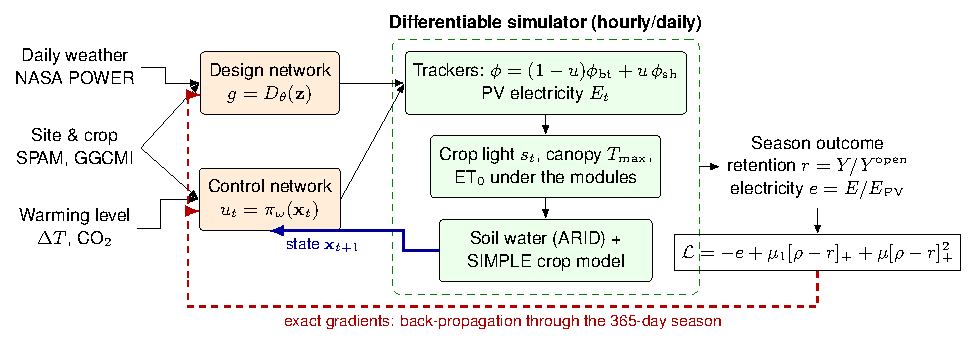
\includegraphics[width=\textwidth]{figures/scheme.pdf}
\caption{Simulator and controller. The array density $g$ of a site is fixed from its historical seasons. A control network maps the daily crop and soil state, the density $g$ and a noisy forecast to the light-sharing level $u_t$. The differentiable simulator converts these decisions into PV electricity, light and microclimate at the crop, soil water and crop growth. The season's electricity and yield retention enter a penalised objective whose exact gradient is back-propagated through the 365-day season.}
\label{fig:scheme}
\end{figure}

\begin{figure}[t]
\centering
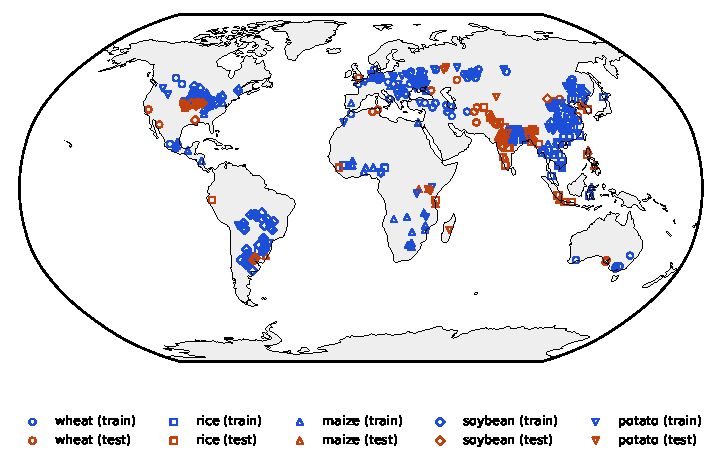
\includegraphics[width=\textwidth]{figures/sites.pdf}
\caption{The 400 crop--site pairs, sampled in proportion to the harvested area of each crop (SPAM 2010). Blue: training sites; orange: geographically held-out test sites of the main split.}
\label{fig:map}
\end{figure}

\begin{figure}[t]
\centering
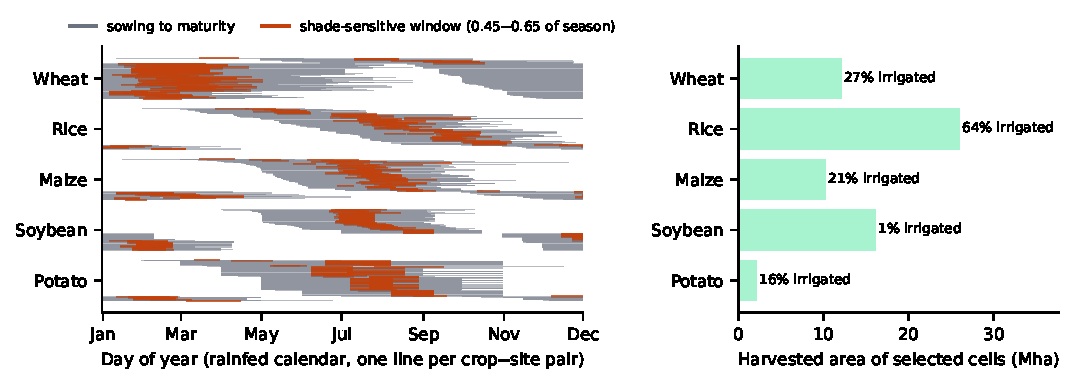
\includegraphics[width=\textwidth]{figures/data_calendar.pdf}
\caption{Agronomic data behind the simulations. Left: crop calendar of the 400 crop--site pairs (GGCMI Phase~3 sowing and maturity dates, one line per pair); the red part marks the window of 0.45 to 0.65 of the season in which the crop model penalises shading through the harvest index (flowering and grain set). Right: harvested area of the selected cells (SPAM 2010) and its irrigated share.}
\label{fig:calendar}
\end{figure}

\subsection{Electricity and food on held-out sites and years}\label{sec:main}
Table~\ref{tab:main} compares the controllers on the 92 held-out crop--site pairs of the main split (95 pairs are held out; pairs without a season whose open-field yield is at least 0.2 t\,ha$^{-1}$ in all four climates are excluded) (seasons sown in 2015--2019), after each site's density has been chosen from its 2001--2014 seasons with the same rule for all controllers. By construction all methods keep the mean yield retention close to 90\% (0.904--0.917), so differences in electricity are differences in the density that each controller can sustain under this floor.

\textbf{Static arrays are the weakest.} Without light sharing, the floor limits the ground coverage to 6\% on average, and arrays produce 217\,MWh\,ha$^{-1}$\,yr$^{-1}$, 16\% of a conventional PV plant per hectare (LER 1.07). Rotating the modules to let light through during the cropping season (seasonal sharing) allows a coverage of 17\% and 397\,MWh\,ha$^{-1}$\,yr$^{-1}$ (LER 1.19). A rule that shares light only while the crop is growing (phenology rule) reaches 465\,MWh\,ha$^{-1}$\,yr$^{-1}$ (LER 1.24). An expert rule that additionally shades the crop on forecast heat or drought days (stress rule) is worse than the phenology rule (LER 1.18): its density is limited to 13\% because it reduces light at times when the floor is most binding.

\textbf{The learned controller is best by a modest margin over the written rule.} SALS sustains a density of 17\% (similar to the phenology rule), produces 510\,MWh\,ha$^{-1}$\,yr$^{-1}$ and reaches an LER of 1.270 at the same retention. Compared with the phenology rule this is +0.038 in LER (95\% CI over sites 0.025--0.053; +10\% electricity) and it is higher at 84\% of the 92 sites (Table~\ref{tab:stats}). Compared with static arrays it is +0.205 (0.176--0.236), with 2.35 times the electricity at 2.9 times the density. The frontier in Fig.~\ref{fig:frontier} shows the same picture at matched densities: the learned policy lies on or slightly above the phenology rule over the whole density range, both lie well above seasonal sharing and the stress rule, and static arrays are far below.

\begin{table}[t]
\centering
\caption{Held-out performance (92 test sites, seasons 2015--2019, canopy cooling $\kappa=1$\,\textdegree C). The density (GCR) of each site is the largest value on the grid $0.05,0.075,\dots,0.5$ at which the method's mean retention in the site's 2001--2014 seasons is $\ge0.9$. $E$: electricity (MWh\,ha$^{-1}$\,yr$^{-1}$); $e$: electricity relative to a conventional PV plant; $r$: mean yield retention; $r_{\mathrm{prod}}$: production-weighted retention; C$_s$ and C$_{\mathrm{site}}$: share of seasons with $r\ge0.9$ and share of sites whose test-season mean $r\ge0.9$ (\%); LER $=r+e$.}
\label{tab:main}
\small
\setlength{\tabcolsep}{4pt}
\begin{tabular}{lcccccccc}
\toprule
Method & GCR & $E$ & $e$ & $r$ & $r_{\mathrm{prod}}$ & C$_s$ & C$_{\mathrm{site}}$ & LER\\
\midrule
\multicolumn{9}{l}{\textit{Baseline}}\\
AV static & 0.06 & 217 & 0.16 & 0.917 & 0.914 & 93 & 96 & 1.07\\
Seasonal sharing & 0.17 & 397 & 0.28 & 0.904 & 0.902 & 69 & 72 & 1.19\\
Phenology rule & 0.17 & 465 & 0.33 & 0.904 & 0.902 & 69 & 75 & 1.24\\
Stress rule & 0.13 & 387 & 0.28 & 0.907 & 0.907 & 76 & 82 & 1.18\\
SALS & 0.17 & 510 & 0.36 & 0.905 & 0.902 & 70 & 74 & 1.27\\
\addlinespace
\multicolumn{9}{l}{\textit{+1.5\,\textdegree C}}\\
AV static & 0.06 & 221 & 0.16 & 0.916 & 0.914 & 93 & 92 & 1.08\\
Seasonal sharing & 0.16 & 393 & 0.28 & 0.905 & 0.903 & 72 & 74 & 1.19\\
Phenology rule & 0.17 & 478 & 0.34 & 0.905 & 0.902 & 68 & 75 & 1.25\\
Stress rule & 0.12 & 377 & 0.27 & 0.908 & 0.908 & 73 & 77 & 1.18\\
SALS & 0.17 & 518 & 0.37 & 0.906 & 0.903 & 68 & 75 & 1.28\\
\addlinespace
\multicolumn{9}{l}{\textit{+2\,\textdegree C}}\\
AV static & 0.06 & 223 & 0.16 & 0.916 & 0.914 & 92 & 93 & 1.08\\
Seasonal sharing & 0.17 & 394 & 0.28 & 0.905 & 0.904 & 72 & 76 & 1.19\\
Phenology rule & 0.17 & 483 & 0.35 & 0.905 & 0.903 & 69 & 74 & 1.25\\
Stress rule & 0.12 & 370 & 0.26 & 0.909 & 0.909 & 75 & 78 & 1.17\\
SALS & 0.17 & 521 & 0.38 & 0.907 & 0.904 & 69 & 75 & 1.28\\
\addlinespace
\multicolumn{9}{l}{\textit{+3\,\textdegree C}}\\
AV static & 0.06 & 231 & 0.17 & 0.915 & 0.914 & 88 & 89 & 1.08\\
Seasonal sharing & 0.17 & 397 & 0.29 & 0.906 & 0.904 & 69 & 75 & 1.19\\
Phenology rule & 0.18 & 499 & 0.36 & 0.905 & 0.902 & 67 & 72 & 1.26\\
Stress rule & 0.11 & 366 & 0.26 & 0.908 & 0.908 & 74 & 77 & 1.17\\
SALS & 0.18 & 540 & 0.39 & 0.907 & 0.904 & 68 & 75 & 1.30\\
\bottomrule
\end{tabular}
\end{table}

\begin{figure}[t]
\centering
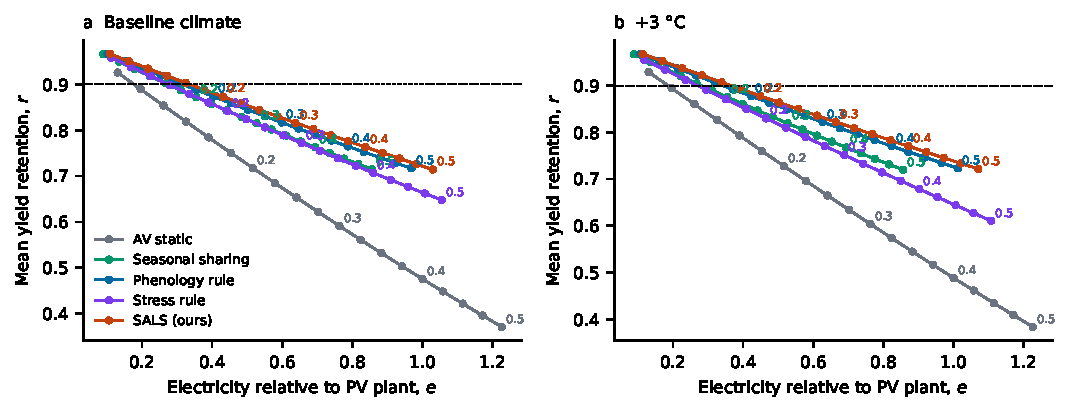
\includegraphics[width=\textwidth]{figures/frontier.pdf}
\caption{Electricity--retention frontiers at identical array densities (labels: GCR) for the held-out sites. Each point is the mean over test seasons at a fixed GCR; the dashed line is the 90\% floor.}
\label{fig:frontier}
\end{figure}

\textbf{What the floor does and does not guarantee.} Enforcing the floor on the historical mean does not guarantee it in every season. In the test seasons, 70\% of SALS seasons have $r\ge0.9$ (phenology rule 69\%, stress rule 76\%, static arrays 93\%), and 2.7\% have $r<0.8$ (1.3\%, 0.9\% and 0.9\%). The lower tail of SALS is therefore slightly heavier than that of the rules: its 10th percentile of $r$ is 0.883, against 0.887, 0.886 and 0.903. Requiring $r\ge0.9$ in at least 80\% of a site's historical seasons (chance-constrained design) raises the season-level compliance to 90--94\% for the light-sharing controllers. It costs about 0.065 in LER for SALS (1.205), which remains the best controller (phenology rule 1.192; Section~\ref{sec:sensitivity}).

\subsection{Robustness}\label{sec:sensitivity}
\textbf{Seeds and splits.} Three training seeds of SALS give LERs of 1.270, 1.268 and 1.269 under the baseline climate and 1.297, 1.298 and 1.297 at +3\,\textdegree C. On two further spatial splits, in which different blocks of sites are held out (training seed 0; the pooled analysis of Table~\ref{tab:ctl} uses three seeds per split), SALS exceeds the phenology rule by 0.047 and 0.041 in LER under the baseline climate and by 0.052 and 0.039 at +3\,\textdegree C (main split, season-pooled: 0.034 and 0.032; the site-level paired contrasts of Table~\ref{tab:stats} are 0.038 and 0.034). In every split SALS ranks first, the phenology rule second and static arrays last.

\textbf{Canopy cooling.} The canopy-cooling coefficient $\kappa$ is the most uncertain microclimate parameter. We repeated the whole protocol, including the historical design step, with $\kappa=0$, 1 and 2\,\textdegree C. Electricity changes with $\kappa$ because cooler canopies tolerate denser arrays (SALS: 475, 510 and 549\,MWh\,ha$^{-1}$\,yr$^{-1}$ under the baseline climate), but the retention is held at 0.905 by the design rule and the ranking is unchanged. SALS exceeds the phenology rule by 0.029, 0.034 and 0.042 in LER under the baseline climate (0.022, 0.032 and 0.051 at +3\,\textdegree C).

\textbf{Which ingredients matter.} Two ablations test the design of SALS at the same training budget. Masking the stress inputs (soil water, ARID, and the maximum temperature, irradiance and ET$_0$ forecasts) leaves the LER unchanged (1.269 vs 1.270 under the baseline climate, 1.297 vs 1.297 at +3\,\textdegree C). Training only on the baseline climate gives 1.268 and 1.291. The improvement over the rules therefore does not depend on stress-aware inputs or on training in warmed climates.

Further sensitivity analyses (floor conditioning, chance-constrained training, forecast errors, layout, rotation limit, harvest-index assumptions and a floor of 66\%) are reported in the Supplementary Material (Section~\ref{sec:extra}); none changes the ranking of the methods (SALS exceeds the written phenology rule by 0.033 to 0.038 LER at floors of 0.80 to 0.95).

\textbf{Tuned rules.} The phenology rule above was written, not tuned, whereas SALS is trained. We therefore tuned its window on the training-block seasons with the same objective as the other rules (electricity at the density where mean retention equals the floor), first on a coarse $4\times3$ grid and then, as a derivative-free baseline, by CMA-ES over a five-parameter schedule (start, end, two ramp widths and a level; three runs of 200 evaluations, Methods). The grid-tuned window starts at 0.15 instead of 0.05 of the thermal-time requirement (Table~\ref{tab:ctl}). Two of the three CMA-ES runs, one started at the grid-tuned window and one at a random point, reached the same almost binary window (all three runs stopped at the generation cap) from 0.20 to 0.93 of the requirement at level 1.00; the third stopped in a worse optimum. Pooled over three splits and 76 distinct crop--site pairs, the grid-tuned window raises LER over the written rule by 0.026 (95\% cluster-bootstrap interval 0.016 to 0.037), the CMA-ES window by 0.036 (0.023 to 0.052) and SALS by 0.044 (0.030 to 0.060), so the optimisation of a window accounts for about 83\% of the margin of SALS over the written rule. SALS exceeds the CMA-ES window by 0.007 LER (0.002 to 0.014), which is 2.4\% more electricity at the designed densities (not at matched retention), and the grid-tuned window by 0.018 (0.011 to 0.025). The remaining margin is small (it covers the pairs only: SALS is the mean of three training seeds per split, whose pooled margins over the CMA-ES window are 0.007, 0.008 and 0.007 (95\% intervals 0.001 to 0.015; results/seed\_margins.csv), and the CMA-ES schedule and the grid window were re-tuned on each split's own training block); it is not explained by the tuning of a window or a ramp, and it cannot come from soil water, forecasts or aridity, because masking them leaves SALS unchanged (Section~\ref{sec:sensitivity}); canopy development and density remain untested. SALS and the CMA-ES window meet the floor in 83\% of seasons, the written, grid-tuned and seasonal rules in 84--85\%; these shares exceed the 69--76\% of Table~\ref{tab:main} because the coarser density grid of this analysis (0.05 against 0.025) selects lower densities, with a mean retention of 0.916 instead of 0.905. Per split, SALS exceeds the CMA-ES window by 0.008 (95\% interval 0.001 to 0.016; 32 pairs), 0.009 (0.001 to 0.022; 26 pairs) and 0.005 ($-0.002$ to $0.012$; 35 pairs), with per-pair medians of 0.001 to 0.002, so the point estimates are positive on every split (the intervals include zero for split 2 and, for some seeds, for split 1) and the margin is concentrated in a few pairs. A site held out in more than one split enters the pooled analysis once, with the mean over its splits, which is why 93 pair-split evaluations give 76 distinct pairs. The design step quantises the density to a grid of 0.05 (about 30\% of the mean density), which is much coarser than the margin. We therefore also compared the controllers on the test seasons at matched mean retention, reading the LER at a retention of 0.90 off the retention--LER curve of each pair (interpolated over the grid): SALS exceeds the CMA-ES window by 0.0033 (95\% interval $-0.0004$ to 0.0071; 73 pairs, those for which the retention curves of all compared methods bracket 0.90, instead of the 76 distinct pairs of the design-based comparison), the grid-tuned window by 0.011 (0.007 to 0.016) and the written rule by 0.036 (0.023 to 0.051). At fixed densities of 0.10 to 0.30 the difference to the CMA-ES window is 0.001 to 0.003 LER, with intervals that include zero. At matched retention the margin over the optimised window is therefore not distinguishable from zero.

\begin{table}[t]
\centering\small
\caption{Rules and the learned controller pooled over the three spatial splits (76 distinct crop--site pairs, every third held-out pair; baseline climate; main shade response; history-based design on a GCR grid with step 0.05, coarser than the 0.025 grid of the main analysis). The grid-tuned window shares light while thermal time lies between 0.15 and 1.0 of the season requirement (best of a $4\times3$ grid on training-block seasons of split~0; the written rule uses 0.05 to 1.0). The CMA-ES schedule has five parameters (start, end, two ramp widths, level) and converged to an almost binary window from 0.20 to 0.93 of the requirement at level 1.00 (two of three runs; see Methods).}\label{tab:ctl}
\begin{tabular}{lcccccc}
\toprule
Method & GCR & $E/E_\mathrm{PV}$ & Retention & Seasons $\ge0.9$ (\%) & Pairs $\ge0.9$ (\%) & LER\\
\midrule
AV static & 0.059 & 0.153 & 0.922 & 95 & 96 & 1.076\\
Seasonal sharing & 0.151 & 0.249 & 0.915 & 84 & 91 & 1.164\\
Stress rule & 0.118 & 0.255 & 0.918 & 83 & 88 & 1.173\\
Phenology rule (written) & 0.154 & 0.292 & 0.916 & 85 & 91 & 1.207\\
Grid-tuned window & 0.161 & 0.317 & 0.916 & 84 & 89 & 1.233\\
CMA-ES optimised window & 0.160 & 0.329 & 0.916 & 83 & 87 & 1.245\\
SALS & 0.161 & 0.335 & 0.916 & 83 & 87 & 1.251\\
\bottomrule
\end{tabular}
\end{table}


\subsection{What the learned policy does}\label{sec:policy}
Averaged over the rainfed test seasons of the main split at a density of 0.3, the light-sharing level of SALS is a smooth function of relative thermal time. It is close to zero in the first 10\% of the thermal time required for maturity, rises through 0.55 at 10--20\%, stays at 0.94--0.99 between 30\% and 70\%, and falls through 0.58 at 80--90\% to about zero at maturity. The plateau overlaps the window in which our crop model penalises shading through the harvest index; we did not test whether this alignment is learned or inherited from the initialisation. The ramps at both ends let the modules produce electricity when additional light is worth least to the crop. Fig.~\ref{fig:trajectory} shows two example seasons. The phenology rule, which is also the initialisation of the network, shares light during the whole growing period. Fine-tuning through the simulator found that sharing can be reduced at the edges of the season: this pattern describes the average policy at a density of 0.3 (the designed mean is 0.17) and we did not test that it causes the gain; the CMA-ES window is almost binary, so a smooth ramp is not needed to reproduce most of it.

\begin{figure}[t]
\centering
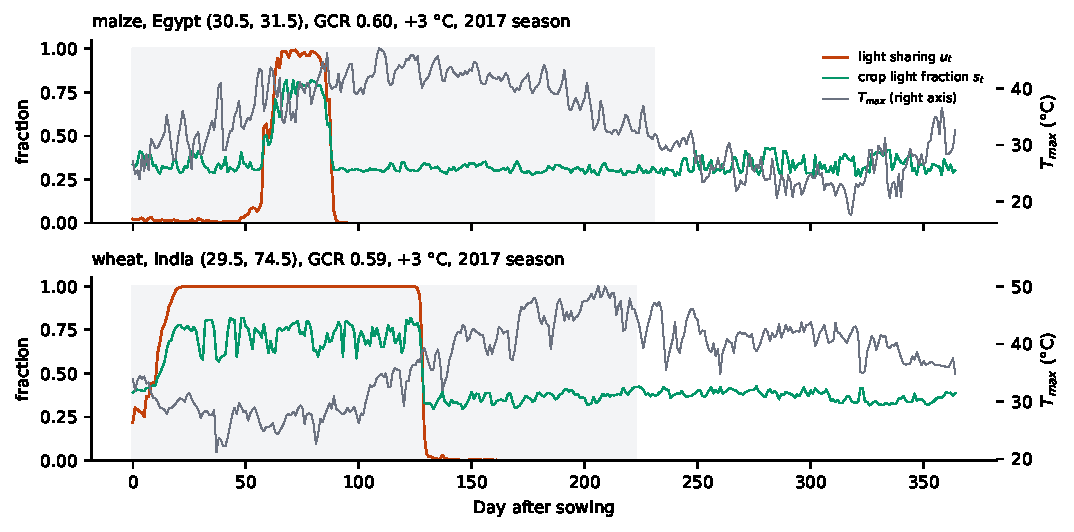
\includegraphics[width=\textwidth]{figures/trajectory.pdf}
\caption{Learned daily control for two test seasons under +3\,\textdegree C, at the density chosen for the site, simulated for the dominant sub-field of the site. Shading marks the cropping window. Orange: light-sharing level $u_t$; green: fraction of open-field irradiance reaching the crop; grey: daily maximum temperature (right axis).}
\label{fig:trajectory}
\end{figure}

The policy also shares less light on days with a forecast heat stress: the mean level is 0.35 on such days against 0.60 (baseline) and 0.51 (+3\,\textdegree C) on other days, and 58--63\% of sites show a lower level on heat days. This cannot be read as a stress response, however. Heat days occur late in the season, when the phenological ramp is already falling, and a policy without any stress input shows a similar contrast (0.37 vs 0.57 in a separate check). The ablation above confirms that stress information does not improve the result.

\subsection{Crops and regions}\label{sec:crops}
The benefit of light sharing differs between crops (baseline climate, SALS). Soybean and maize tolerate the densest arrays (GCR 0.24 and 0.19; 691 and 577\,MWh\,ha$^{-1}$\,yr$^{-1}$; LER 1.41 and 1.30), potato follows (0.19; 542; 1.31), and rice and wheat are the most restrictive (0.13 and 0.15; 395 and 428; 1.20 for both). The stress rule has a lower LER for every crop (1.26 for soybean, 1.14--1.21 for the others).

The floor is not met evenly. Production-weighted retention is 0.888 for soybean and 0.898 for maize, below 0.9, because high-yielding seasons lose more than low-yielding ones. Regionally, Latin America and Oceania (4 sites) combine the highest density (GCR 0.41) and electricity (1090\,MWh\,ha$^{-1}$\,yr$^{-1}$) with a production-weighted retention of only 0.862. Africa and the Middle East (8 sites) reach 0.894, and only 63\% of their sites keep a mean retention of at least 0.9. South Asia, the region with the most sites (39), reaches 0.902 (67\% of sites) at a density of 0.14. The regional figures rest on 4 to 39 sites and are uncertain: the 95\% site-bootstrap intervals of the production-weighted retention are 0.841 to 0.897 for Latin America and Oceania, 0.868 to 0.908 for Africa and the Middle East and 0.898 to 0.905 for South Asia, and the share of sites that meet the floor has intervals of 25 to 88\% (Africa and the Middle East), 25 to 100\% (Latin America and Oceania) and 51 to 79\% (South Asia; results/by\_region\_ci.csv). Only the retention deficit of Latin America and Oceania (four sites) lies outside the interval of South Asia, that of Africa and the Middle East overlaps it, and no multiplicity adjustment was made, so the region comparison is an indication and not a finding. The pooled retention hides differences between crops (soybean 0.888, maize 0.898), so a floor enforced per site would plausibly need a crop- and site-specific design step.

\subsection{Model behaviour and validation}\label{sec:shade}
\textbf{PV output.} The simulated specific yield of an isolated tracker row agrees with PVGIS 5.2 \citep{pvgis} at 29 sites with $r=0.971$, a mean bias of $-4.9$\% and a mean absolute deviation of 5.5\% (Section~\ref{sec:sim}). At higher ground coverage the shading and diffuse-transposition model was compared with pvlib \citep{holmgren2018} (infinite-sheds model with isotropic sky and backtracking, driven by the same hourly irradiance and sun position at 12 sites spanning the latitudes of the data set, year-round). The simulated plane-of-array irradiance is 0.4\% above pvlib at $g=0.05$ and 0.7, 1.4, 2.1, 2.6 and 3.0\% above it at $g=0.1$, 0.2, 0.3, 0.4 and 0.5 (site ranges within 0.1 to 1.0 points of these means). The loss relative to a sparse array is therefore underestimated: 2.8\% instead of 4.4\% at $g=0.3$ and 6.3\% instead of 8.7\% at $g=0.5$, which favours dense arrays by about 1.5 to 2.5 points of electricity in this range. To gauge the effect of this bias we multiplied the electricity of every method, and that of the reference plant ($g=0.4$) that defines the LER, by the ratio of the pvlib to the simulated relative irradiance (0.996 at $g=0.1$, 0.990 at 0.2, 0.983 at 0.3, 0.978 at 0.4 and 0.974 at 0.5; retention and hence the designed densities do not depend on electricity). The ratio was obtained for backtracking and is assumed to hold for the light-sharing rotations, and we did not test whether the ground-side shade table carries a related bias that would change retention. As a sensitivity, not a proven bound, we also applied the square of the ratio. The LER of the light-sharing methods rises by 0.003 to 0.004 (0.008 with the squared ratio; SALS 1.251, 1.255, 1.259) because the reference plant is corrected more than the sparser arrays, the LER of static arrays by 0.003 (0.007), and the margins of SALS over the written rule and the CMA-ES window change by at most 0.0003 (0.044 and 0.007). The break-even prices of the arrays rise by about 0.8 USD\,MWh$^{-1}$ for the light-sharing methods and 0.1 for static arrays (1.5 and 0.2 with the squared ratio; SALS 73.4, 74.2; static arrays 58.6, 58.7), that of the plant by 1.1 (48.8; 64.1 at equal capex), the net value of SALS at 90 USD\,MWh$^{-1}$ falls from 7.6 to 7.2 (6.8) kUSD\,ha$^{-1}$\,yr$^{-1}$, and the ranking of the methods does not change (results/pvbias.csv). The PVGIS level bias of $-4.9$\% was not propagated.

\textbf{Shade response.} Fig.~\ref{fig:shade} shows the simulated relative yield of rainfed crops under static arrays as a function of the season-mean shading of the crop. Yield declines close to proportionally with shading: 84--89\% relative yield at 12\% shading, 70--78\% at 25\%, 57--67\% at 37\% and 35--46\% at 57\%. Wheat loses most and potato and maize least. This response is steeper than the \emph{less than proportional} losses that \citet{laub2022} report for small shade levels of C3 cereals and tubers, and it does not reproduce their finding that maize and grain legumes are more shade sensitive than C3 cereals. In the simulator, shading also relieves heat and drought in rainfed maize and soybean, which offsets the higher harvest-index penalty we assigned to them. The absolute effect of shading on each crop is therefore uncertain (Section~\ref{sec:limits}).

\begin{figure}[t]
\centering
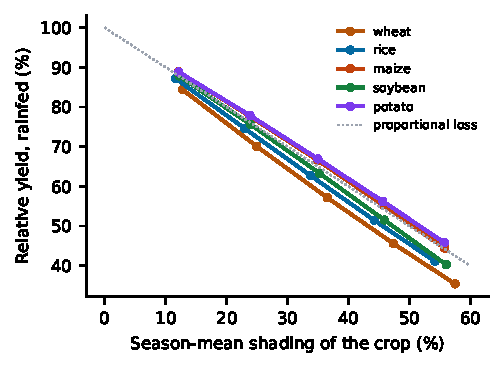
\includegraphics[width=0.6\textwidth]{figures/shade_response.pdf}
\caption{Simulated relative yield of rainfed crops under static arrays (GCR 0.1--0.5) against season-mean shading of the crop, baseline climate, held-out sites. The dotted line is proportional loss.}
\label{fig:shade}
\end{figure}

\textbf{Comparison with field trials.} We fitted one radiation-use compensation coefficient per crop to the yield--shading curves of \citet{laub2022} using training-block sites only (Methods, calibration script in the repository). The fit changed wheat and rice only (coefficients 0.4 and 0.1) because the proportional model already lies within about 0.02 of the C3-cereal and tuber curves, and it cannot lower the maize and legume responses below the proportional case (root-mean-square error 0.16 for maize and 0.08 for soybean). Against field trials (not independent of the choice of ensemble, Table~\ref{tab:fieldval}) the model underestimates retained yield: rice 0.79 against 0.84 \citep{gonocruz2021}, wheat and potato 0.74 and 0.72 against 0.81--0.82 in the worse season of \citet{weselek2021} (and above 1 in the better one), and maize 0.70--0.75 against 0.83--0.91 at 30--35\% shading \citep{ramosfuentes2023}, where harvest index was not affected by shade. The model is therefore conservative for food retention with respect to these trials, except for the stronger maize losses of the meta-analysis. Table~\ref{tab:variants} shows the consequence for the design results: with the calibrated response the allowed density and the LER of every method rise (phenology rule 1.28 against 1.23), and with a response fitted to the field trials the LER of the phenology rule is 1.62. The phenology rule is the best method in all three cases, and light sharing adds LER $+0.17$, $+0.19$ and $+0.30$ over static arrays (conservative, calibrated, field-fitted); only the order of the seasonal and stress rules changes. The absolute gains for rice, wheat and potato are thus conservative with respect to these trials; for maize and soybean the meta-analysis points the other way (Section~\ref{sec:mlresults}).

\begin{table}[t]
\centering\small
\caption{Simulated relative yield at the shading of published field trials (static arrays, training-block sites). Observed values: mean of reported seasons; for wheat and potato the two-year range is $-18.7$ to $+2.7$\% and $-18.2$ to $+11$\%.}\label{tab:fieldval}
\begin{tabular}{lcccc}
\toprule
Trial & Shading & Observed & Conservative & Calibrated\\
\midrule
Rice, \citet{gonocruz2021} & 0.25 & 0.84 & 0.77 & 0.79\\
Wheat, \citet{weselek2021} & 0.30 & 0.81 & 0.66 & 0.74\\
Potato, \citet{weselek2021} & 0.30 & 0.82 & 0.72 & 0.72\\
Maize, \citet{ramosfuentes2023} (DAV) & 0.35 & 0.83 & 0.70 & 0.70\\
Maize, \citet{ramosfuentes2023} (half) & 0.30 & 0.91 & 0.75 & 0.75\\
Maize, \citet{ramosfuentes2023} (full) & 0.50 & 0.70 & 0.54 & 0.54\\
\bottomrule
\end{tabular}
\end{table}


\subsection{A shade-response model learned from field data}\label{sec:mlresults}
Cross-validation by study shows what the data can and cannot support (Tables~\ref{tab:mlcv} and~\ref{tab:mlcvtype}). Over all 339 shaded observations the root-mean-square error of a held-out study falls from 0.43 for proportional loss $y=1-s$ to 0.37 for one curve for all crops and to 0.31 for crop-type curves, but this gain comes from crop types that the simulator does not represent (berries, forages, fruits and vegetables: 0.53 to 0.36). For the four crop types that the simulator uses, the learned curves are not better than proportional loss: the error is 0.222 against 0.220 pooled (difference $+0.002$, 95\% interval $-0.023$ to $+0.030$), 0.187 against 0.214 for C3 cereals, and slightly worse for maize, grain legumes and tubers. Partial pooling is as good as separate curves (0.312 against 0.313) and the covariates add almost nothing (0.311). Gradient-boosted trees on the same inputs are worse (0.321) than the parametric model. The error of 0.22 for the four crop types is large: yields of a new study differ from the learned curve by about 20 percentage points, which is the between-study spread that a design under uncertainty has to cover. Crop type is the information that transfers between studies, and none of the covariate effects on $\log\beta$ is clearly different from zero (irradiation $-0.10$, 90\% interval $-0.32$ to $0.09$; subtropical zone $-0.37$, $-0.73$ to $0.07$; intercropping $0.16$, $-0.48$ to $0.45$). The estimated effect of solar-panel shade is not interpretable, because all 46 panel observations are of leafy vegetables, mainly lettuce, and the effect is confounded with crop type.


The learned curves show a clear ordering of crop types (Fig.~\ref{fig:datashade} and Table~\ref{tab:mlcurves}). At 20\% shading C3 cereals and tubers lose less than proportionally (relative yield 0.93), whereas maize (0.73) and grain legumes (0.71) lose more; at 40\% shading the values are 0.72 and 0.71 against 0.42 and 0.40. Intervals are wide for maize ($0.27$--$0.59$ at 40\%) and for tubers, which rest on two studies. The simulator's responses are close to the data for cereals and potato but, under both calibrated ensembles, too mild for maize at 40\% shading (0.75 for E2 against 0.42 in the data); for soybean the E2 value (0.48) lies within the interval of the data (0.40, 80\% interval 0.34--0.53). The calibration cannot lower the maize response further, because the simulated shading also relieves heat and drought stress and the compensation and harvest-index parameters are bounded below at zero. The field trials of maize are also milder than the meta-analysis: \citet{ramosfuentes2023} report a harvest index unaffected by shade, and \citet{sekiyama2019} a yield $5.6$\% above the control under a low-density stilt-mounted array in one season at one site. For maize and soybean the direction of the bias is uncertain, and the gains reported in this paper are possibly overestimated.

\begin{figure}[t]
\centering
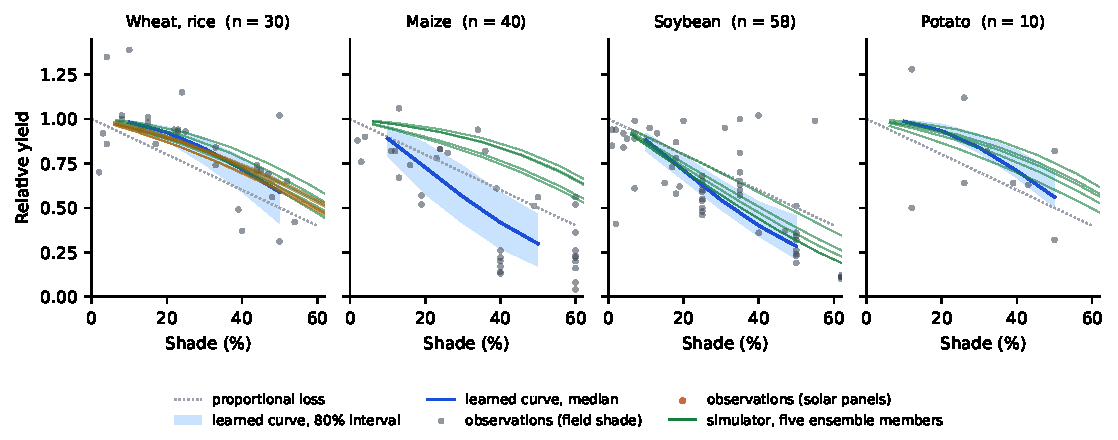
\includegraphics[width=\textwidth]{figures/data_shade.pdf}
\caption{Yield response to shade: the observations of the meta-analysis \citep{laub2022} for the crop types that the simulator represents (grey: field shade; orange: solar-panel shade), the hierarchical curve learned from them (median and 80\% bootstrap interval over studies) and the simulated response of each of the five members of ensemble E2 (green, static arrays, baseline climate; wheat and rice in green and brown). The curve of C3 cereals stands for rice, for which the data set has no study. For maize the simulator is clearly milder than the data.}
\label{fig:datashade}
\end{figure}

\begin{table}[t]
\centering\small
\caption{Relative yield at 20\% and 40\% shading: data-driven model (median and 80\% bootstrap interval over studies; crop-type curve, covariates at their reference values: mean irradiation, temperate zone, no solar-panel shade, no intercropping) and simulator under the two calibrated ensembles (mean of members; E1 fitted to hand-read curves, E2 fitted to the data-driven curves). The data-driven curve of rice is that of C3 cereals (no rice in the data set). Observations and studies: C3 cereals 41/10, maize 51/10, grain legumes 76/14, tubers 12/2.}\label{tab:mlcurves}
\begin{tabular}{llcccc}
\toprule
Crop & Shading & Data-driven & Simulator, E1 & Simulator, E2 & Proportional\\
\midrule
Wheat & 20\% & 0.93 [0.88, 0.96] & 0.88 & 0.92 & 0.80\\
Wheat & 40\% & 0.72 [0.59, 0.78] & 0.70 & 0.77 & 0.60\\
Rice & 20\% & 0.93 [0.88, 0.96] & 0.85 & 0.90 & 0.80\\
Rice & 40\% & 0.72 [0.59, 0.78] & 0.66 & 0.73 & 0.60\\
Maize & 20\% & 0.73 [0.58, 0.86] & 0.86 & 0.90 & 0.80\\
Maize & 40\% & 0.42 [0.27, 0.59] & 0.69 & 0.75 & 0.60\\
Soybean & 20\% & 0.71 [0.65, 0.79] & 0.77 & 0.74 & 0.80\\
Soybean & 40\% & 0.40 [0.34, 0.53] & 0.53 & 0.48 & 0.60\\
Potato & 20\% & 0.93 [0.92, 0.97] & 0.88 & 0.92 & 0.80\\
Potato & 40\% & 0.71 [0.67, 0.83] & 0.73 & 0.79 & 0.60\\
\bottomrule
\end{tabular}
\end{table}


\subsection{Learning under shade-response uncertainty}\label{sec:uncertain}
\textbf{Calibration.} Gradient descent through the simulator fitted the five crops to the data-driven curves and the field trials (ensemble E2, Table~\ref{tab:posterior}). The data identify two features: the harvest index of maize is hardly affected by shade (multiplier $0.16\pm0.13$, $c\approx0.14$), as observed by \citet{ramosfuentes2023}, and soybean is more shade sensitive than the cereals (compensation $0.05$, harvest-index multiplier $1.66$), as in \citet{laub2022}. Wheat has the largest compensation ($0.91\pm0.31$) and the largest uncertainty; the compensation is an effective parameter that absorbs diffuse-light and light-saturation effects that the simulator does not model explicitly, not a physical value.


\textbf{Learned controllers.} Controllers were evaluated under four fixed responses on 21 crop--site pairs of split~0 with one training seed, so the intervals below, which are cluster bootstraps over pairs of per-pair mean LER differences, do not include seed or split variation (Table~\ref{tab:robust} gives season means, which differ slightly). Under every response SALS, trained on the proportional response, is better than the written phenology rule: by $+0.019$ ($+0.007$ to $+0.039$), $+0.024$ ($+0.009$ to $+0.046$), $+0.038$ ($+0.018$ to $+0.062$) and $+0.015$ ($+0.001$ to $+0.037$) LER under the proportional, calibrated, field-fitted and harsh responses. It is also above the grid-tuned window and the CMA-ES optimised window, but by less: 0.005 to 0.018 and 0.005 to 0.010 LER, with intervals that exclude zero for the grid-tuned window under 3 of the four responses and for the CMA-ES window under none. Training on the narrow ensemble E1 did not change this: SALS-robust differs from SALS by $-$0.005 to $+$0.003 (intervals contain zero except for one response) and SALS-adaptive, which sees the measured biomass ratio, by $-$0.010 to $+$0.007. Training on the wider ensembles did not help either (the robust controllers fall below SALS even under responses inside their training ensemble, which may point to under-training with our budget of 300 steps): SALS-robust on E2 and E3 and SALS-adaptive on E3 are below SALS by 0.014, 0.017, 0.017 LER under the proportional response, 0.017, 0.021, 0.020 under the calibrated response, 0.004, 0.005, 0.011 under the field-fitted response (intervals contain zero) and 0.008, 0.014, 0.017 under the harsh response; the intervals exclude zero in 7 of the 9 comparisons for the proportional, calibrated and harsh responses. The E3 robust controller is not distinguishable from the written rule ($+$0.001 to $+$0.032) under any response (all intervals contain zero). With one seed and 21 pairs these controllers therefore did not retain the margin of SALS within our training budget; a controller that must perform across plausible responses is less specialised, but a larger budget or more seeds could change this. The feedback rule is worse than the written rule by 0.026--0.058 LER under every response (intervals exclude zero). A plausible reason is that the biomass ratio does not reveal the harvest-index loss from shading around flowering, but we did not test this explanation.

\begin{table}[t]
\centering\small
\caption{Land-equivalent ratio of rules and learned controllers under four true shade responses, with the array density designed under the true response (split~0, baseline climate, floor $\rho=0.9$, every sixth held-out pair, 21 pairs, coarse GCR grid, one training seed; season means, so differences differ slightly from the pair-level intervals in the text). SALS is trained on the proportional response; robust controllers are trained on random members of ensemble E1, E2 or E3 (adaptive: with the measured biomass ratio). The proportional and harsh responses lie outside the ensembles.}\label{tab:robust}
\begin{tabular}{lcccc}
\toprule
Method & Proportional & Calibrated & Field-fitted & Harsh\\
\midrule
AV static & 1.052 & 1.059 & 1.254 & 1.037\\
Seasonal sharing & 1.133 & 1.156 & 1.385 & 1.097\\
Stress rule & 1.129 & 1.160 & 1.406 & 1.086\\
Feedback rule & 1.139 & 1.164 & 1.392 & 1.089\\
Phenology rule (written) & 1.164 & 1.190 & 1.456 & 1.122\\
Grid-tuned window & 1.170 & 1.199 & 1.472 & 1.129\\
CMA-ES optimised window & 1.173 & 1.198 & 1.479 & 1.125\\
SALS & 1.178 & 1.209 & 1.489 & 1.132\\
SALS-robust, E1 & 1.179 & 1.204 & 1.491 & 1.127\\
SALS-adaptive, E1 & 1.176 & 1.202 & 1.495 & 1.124\\
SALS-robust, E2 & 1.165 & 1.192 & 1.483 & 1.126\\
SALS-robust, E3 & 1.163 & 1.191 & 1.481 & 1.121\\
SALS-adaptive, E3 & 1.164 & 1.191 & 1.475 & 1.118\\
\bottomrule
\end{tabular}
\end{table}


\textbf{Design under uncertainty.} The design step is a second source of risk, and compliance there is sensitive to the assumed response (Tables~\ref{tab:design} and~\ref{tab:ooe}, Fig.~\ref{fig:designfrontier}). The designs below are evaluated by leaving one ensemble member out as the truth and using the other four, so that the truth never enters the design. Pooled over the three spatial splits (76 distinct crop--site pairs), a density chosen under the mean response of E2 leaves 70\% of the pairs at the floor when the true response is another plausible one, against 87\% for an oracle design (E3: 71\% and 85\%). Choosing the density so that the floor is met in at least 75\% of the other members raises compliance by $+7.9$ points under E2 (95\% cluster-bootstrap interval 4.5 to 11.6) and $+7.9$ under E3 (3.9 to 12.1), at a cost of 0.031 and 0.025 in LER. Raising the floor used in the design from 0.90 to 0.92 under the mean response does more: $+18.0$ points (13.4 to 22.6) at 0.068 LER under E2 and $+14.3$ points (9.5 to 19.2) at 0.056 under E3, and the shortfall is smaller (mean over pairs of the maximum of zero and 0.9 minus retention: 0.0022 against 0.0045 for the quantile rule under E2). The two kinds of rule lie on one frontier (Fig.~\ref{fig:designfrontier}). Interpolating the margin frontier (floors 0.90 to 0.96) at the compliance of the ensemble rules, the LER of the margin minus that of the rule is +0.001 (-0.009 to +0.012) for the rule with 75\% of the other members and +0.003 (-0.016 to +0.021) for the rule with all of them under E2, and -0.006 (-0.019 to +0.005) and +0.024 (-0.011 to +0.058) under E3 (95\% intervals). We find no detectable difference, but the intervals (down to $-0.02$ and up to $+0.06$ LER) are too wide to establish equivalence. The ensemble is thus useful for sizing the margin (0.02 to 0.04 above the floor for 85--97\% of the pairs), not for replacing it. None of these rules is safe outside the ensemble (Table~\ref{tab:ooe}): under the proportional, calibrated and harsh responses the mean-response design leaves 7--17\% of the pairs at the floor, a floor of 0.92 or the ensemble rules 12--33\%, a floor of 0.94 29--47\% and a floor of 0.96 51--78\%, at a cost of about 0.2 LER, whereas the field-fitted response, which lies within the range spanned by the ensembles, is handled well by every rule (80--99\%) except the mean-response design (68--79\%). Outside the ensemble the shortfall of the pairs below the floor is also large: under E2 the mean shortfall per pair (maximum of zero and 0.9 minus retention) is 0.075, 0.060 and 0.104 for the mean-response design under the proportional, calibrated and harsh responses, against 0.053, 0.038 and 0.078 for a floor of 0.92 and 0.012, 0.007 and 0.024 for a floor of 0.96. Across the five members of an ensemble, the standard deviation of the simulated relative yield of a crop (static arrays, baseline climate, held-out sites of split~0) is 0.02 to 0.04 at 20\% shading and 0.02 to 0.06 at 40\% under E2, and 0.02 to 0.09 and 0.03 to 0.15 under E3 (largest for soybean and potato; ranges between the extreme members up to 0.36), against a leave-one-study-out error of 0.22 for new studies. The two quantities differ (a spread of curves against an error over observations), but the ensembles are narrower than the between-study spread for all crops except, possibly, soybean under E3. The pooled shares hide large differences between crops (Table~\ref{tab:ooecrop}, E2, 10 to 20 pairs per crop). Under the proportional, calibrated and harsh responses the design under the mean response and the rule that requires 75\% of the members leave no wheat, rice or potato pair at the floor and at most 12\% of the maize pairs (a floor of 0.92 raises this to at most 10\% of the rice pairs and 18\% of the maize pairs), whereas 90 to 100\% of the soybean pairs meet it, because the ensemble already contains steep soybean responses (the oracle design reaches 90\% for soybean and 65 to 100\% for the other crops). Even a floor of 0.96 leaves 0 to 12\% of the wheat pairs at the floor under the harsh and proportional responses and 42\% of the potato pairs. The out-of-ensemble failure is thus a failure for cereals, tubers and maize, and the pooled values of 7 to 33\% mix crops that fail completely with a crop that does not fail. The guarantee therefore holds only within the range of responses that the ensemble spans; we did not test an ensemble that spans the proportional and harsh responses, which would protect against them at a higher cost in LER.

\begin{table}[t]
\centering\small
\caption{Array design under shade-response uncertainty (ensemble E2). Truth: each of five ensemble members in turn. Designs: oracle (density chosen under the truth), ensemble mean (density chosen under the mean response) and uncertainty-aware (density chosen so that the floor is met in at least 75\% of the \emph{other} four members). Means over the five held-out members; retention is the mean season retention, site compliance the share of sites whose mean retention is $\ge0.9$.}\label{tab:design}
\begin{tabular}{llccccc}
\toprule
Design & Method & GCR & Retention & Seasons $\ge0.9$ (\%) & Sites $\ge0.9$ (\%) & LER\\
\midrule
oracle & Phenology rule & 0.261 & 0.913 & 76 & 79 & 1.412\\
oracle & SALS & 0.256 & 0.912 & 73 & 73 & 1.438\\
ensemble mean & Phenology rule & 0.272 & 0.907 & 60 & 63 & 1.427\\
ensemble mean & SALS & 0.262 & 0.909 & 62 & 62 & 1.446\\
uncertainty-aware & Phenology rule & 0.245 & 0.918 & 73 & 73 & 1.385\\
uncertainty-aware & SALS & 0.238 & 0.917 & 69 & 71 & 1.406\\
\bottomrule
\end{tabular}
\end{table}

\begin{table}[t]
\centering\small
\caption{Design rules outside the ensemble: share of crop--site pairs (\%) with mean retention $\ge0.9$ under four fixed responses (P proportional, C calibrated to the meta-analysis, F field-fitted, H harsh), phenology rule, three splits pooled (76 distinct pairs). Designs use the whole ensemble E2 or E3 (five members and their mean); the oracle uses the true response. LER in the last two columns is the mean over the four responses; the oracle rows are identical for E2 and E3 because the oracle uses the true response.}\label{tab:ooe}
\begin{tabular}{lcccccccccc}
\toprule
 & \multicolumn{4}{c}{E2} & \multicolumn{4}{c}{E3} & \multicolumn{2}{c}{LER}\\
Design & P & C & F & H & P & C & F & H & E2 & E3\\
\midrule
oracle (true response) & 91 & 89 & 87 & 84 & 91 & 89 & 87 & 84 & 1.283 & 1.283\\
mean response & 13 & 13 & 68 & 12 & 13 & 17 & 79 & 7 & 1.435 & 1.448\\
floor met in 75\% of members & 16 & 16 & 80 & 12 & 22 & 25 & 93 & 13 & 1.384 & 1.397\\
floor met in all members & 17 & 17 & 80 & 12 & 29 & 32 & 93 & 16 & 1.348 & 1.336\\
floor 0.92 under mean response & 17 & 20 & 86 & 12 & 29 & 33 & 91 & 20 & 1.376 & 1.399\\
floor 0.94 under mean response & 45 & 47 & 97 & 34 & 45 & 45 & 97 & 29 & 1.303 & 1.345\\
floor 0.96 under mean response & 63 & 78 & 99 & 54 & 58 & 63 & 99 & 51 & 1.220 & 1.264\\
\bottomrule
\end{tabular}
\end{table}


\begin{figure}[t]
\centering
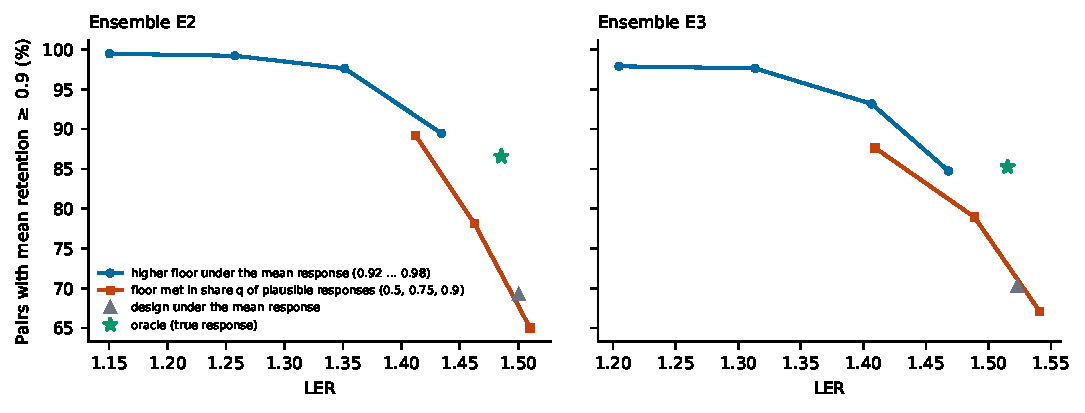
\includegraphics[width=\textwidth]{figures/design_frontier.pdf}
\caption{Share of crop--site pairs at the floor against LER for the phenology rule under design rules for shade-response uncertainty (leave-one-member-out, three splits, 76 pairs): a higher floor under the mean response (blue; the first point is the design under the mean response) and a floor met in a share of the other members (orange), with the oracle design (green).}
\label{fig:designfrontier}
\end{figure}


\subsection{Economics of light sharing}\label{sec:cost}
All figures in this section follow from the assumed parameters of Table~\ref{tab:costparams} and should be read as a sensitivity analysis, not a forecast. The economics are dominated by the capacity installed, not by the crop (Table~\ref{tab:cost}): the annuity and operating cost of the modules is 11--32 kUSD per hectare and year, whereas the crop revenue lost is about 0.3 kUSD, so a method is worth what it earns per installed watt. With the densities designed for the floor, static arrays earn $+0.3$ kUSD\,ha$^{-1}$\,yr$^{-1}$ at 60\,USD\,MWh$^{-1}$ and break even at 59, whereas all light-sharing methods lose money at that price ($-3$ to $-10$ kUSD) and break even at 70 (stress rule), 73 (SALS), 73 (CMA-ES window), 77 (grid-tuned window), 80 (written rule) and 92 (seasonal sharing) USD\,MWh$^{-1}$. The 95\% cluster-bootstrap intervals over pairs are 56--61 for static arrays, 69--76 for SALS, 70--77 for the CMA-ES window and 75--84 for the written rule, and 46--50 for the plant (break-even prices of SALS and the CMA-ES window differ by $-0.4$, $-1.1$ to 0.4); they cover the sampling of pairs and not the cost assumptions. At 90 USD\,MWh$^{-1}$ static arrays (6.3 kUSD) are better than the written (4.0) and grid-tuned (5.5) rules, close to the CMA-ES window (7.3) and worse than SALS (7.6), which overtakes static arrays above about 85 USD\,MWh$^{-1}$; the difference between SALS and static arrays at 90 USD\,MWh$^{-1}$ is $+1.3$ kUSD (95\% interval $-0.04$ to $2.7$, 76 pairs) and not distinguishable from zero, whereas SALS exceeds the CMA-ES window by 0.3 ($-0.1$ to 0.8, not distinguishable from zero), the grid-tuned window by 2.1 (1.6 to 2.7) and the written rule by 3.6 (2.8 to 4.5). A conventional plant that replaces the crop breaks even at 48 USD\,MWh$^{-1}$ and is more profitable than SALS above about 35 USD\,MWh$^{-1}$ and than static arrays above about 46 (16 kUSD at 60, 94 kUSD at 120, against $-6$ and 21 for SALS); below 48 the plant loses money, and below about 46 static arrays lose least of the options (at 30 USD\,MWh$^{-1}$: plant $-23.2$, SALS $-18.7$, static $-5.7$ kUSD). These plant results rest on the assumed capex of 0.75 USD\,Wp$^{-1}$ for a ground-mounted tracker plant against 1.0 for the elevated agrivoltaic structure; the higher agrivoltaic capex is in line with a levelised cost of electricity that is 38\% higher than that of ground-mounted PV in a techno-economic study \citep{schindele2020}; with equal capex the plant breaks even at about 63 USD\,MWh$^{-1}$ and overtakes SALS above about 58 and static arrays above about 64 (results/pvbias.csv). Per megawatt-hour, the electricity of SALS costs about 73 USD including the crop lost, against 48 USD for the plant, a difference of 25 USD\,MWh$^{-1}$. A premium of that size would equalise the unit cost but not the profit per hectare, because a hectare of plant produces three times as much electricity (1306 against 438 MWh): for the same electricity as one hectare of plant, SALS needs about three hectares of array, which costs about 25 USD\,MWh$^{-1}$ more including the crop lost but keeps about 90\% of the yield of that cropland; relative to the plant, SALS would need a premium of about 49 USD\,MWh$^{-1}$ at a market price of 60 and about 109 at 90 to match its profit per hectare, and only about 13 at 60 (none above 73) to match the open field. The sensitivity is large (Table~\ref{tab:costsens}), and the ranking of static arrays and light sharing flips with the module cost (at 1.5 USD\,Wp$^{-1}$ static arrays are better than SALS, at 0.7 SALS leads by 7 kUSD): at 90 USD\,MWh$^{-1}$ the net value of SALS changes from $+17$ to $-8$ kUSD between module costs of 0.7 and 1.5 USD\,Wp$^{-1}$, whereas crop prices matter little.

Because the density was designed for the floor and not for profit, we also let each site choose, among the densities that meet the floor in its history, the one that maximises its historical net value (sites where none pays stay open field; Fig.~\ref{fig:costopt}). Then no method pays at 30--40 USD\,MWh$^{-1}$; at 60 14--59\% of the pairs install an array (none for seasonal sharing) and the net values are small (static arrays 0.9, SALS 0.3 kUSD); static arrays are the best option up to about 75 USD\,MWh$^{-1}$, SALS overtakes them at about 75 (4.9 against 4.3 at 80, 8.3 against 6.3 at 90, 20.7 against 12.3 at 120), the CMA-ES window at about 78, the stress rule at about 81, the grid-tuned window at about 87 and the written rule at about 97. The value of control is therefore real but depends on a high price: at 90 USD\,MWh$^{-1}$ and with profit-optimal densities SALS exceeds the CMA-ES window by 0.4 kUSD\,ha$^{-1}$\,yr$^{-1}$ (95\% cluster-bootstrap interval 0.01 to 0.8), the grid-tuned window by 1.7 (1.2 to 2.2), the written rule by 2.8 (2.0 to 3.6) and static arrays by 2.0 (0.8 to 3.3); the CMA-ES window exceeds static arrays by about 1.6 (0.4 to 2.8), so most of the value of control is obtained with a well-optimised rule.

\begin{table}[t]
\centering\small
\caption{Assumed economic parameters (illustrative, not data). Ranges used in the sensitivity analysis are in parentheses.}\label{tab:costparams}
\resizebox{\ifdim\width>\linewidth\linewidth\else\width\fi}{!}{\begin{tabular}{ll}
\toprule
Parameter & Value\\
\midrule
Electricity price & 60 USD MWh$^{-1}$ (30--120)\\
Capex, AV single-axis tracker plant & 1.0 USD Wp$^{-1}$ (0.7--1.5)\\
Capex, conventional tracker plant & 0.75 USD Wp$^{-1}$\\
Discount rate, lifetime, O\&M & 6\% (4--8\%), 25 years, 1.5\% of capex per year\\
Installed capacity & 2.1 MWp per hectare of module area share $g$ (0.21 kWp m$^{-2}$)\\
Crop price per tonne of dry matter & wheat 290, rice 400, maize 250, soybean 520, potato 1000 USD (0.5--2$\times$)\\
\bottomrule
\end{tabular}}
\end{table}

\begin{table}[t]
\centering\small
\caption{Illustrative annual economics per hectare (76 crop--site pairs, three splits, main shade response, baseline climate; parameters in Table~\ref{tab:costparams}). Net value is relative to the open field (crop costs unchanged) in kUSD\,ha$^{-1}$\,yr$^{-1}$ at three electricity prices; break-even is the price at which the net value is zero. The conventional plant replaces the crop.}\label{tab:cost}
\resizebox{\ifdim\width>\linewidth\linewidth\else\width\fi}{!}{\begin{tabular}{lccccccc}
\toprule
Method & $E$ (MWh) & Capex annuity + O\&M & Crop loss & Net at 60 & Net at 90 & Net at 120 & Break-even (USD/MWh)\\
\midrule
AV static & 200 & 11.5 & 0.27 & 0.3 & 6.3 & 12.3 & 59\\
Seasonal sharing & 326 & 29.6 & 0.31 & -10.3 & -0.5 & 9.2 & 92\\
Stress rule & 336 & 23.2 & 0.30 & -3.3 & 6.8 & 16.9 & 70\\
Phenology rule (written) & 382 & 30.1 & 0.30 & -7.5 & 4.0 & 15.4 & 80\\
Grid-tuned window & 415 & 31.6 & 0.31 & -7.0 & 5.5 & 17.9 & 77\\
CMA-ES optimised window & 428 & 31.0 & 0.30 & -5.6 & 7.3 & 20.1 & 73\\
SALS & 438 & 31.6 & 0.31 & -5.6 & 7.6 & 20.7 & 73\\
Conventional PV plant & 1306 & 58.7 & 3.60 & 16.0 & 55.2 & 94.4 & 48\\
\bottomrule
\end{tabular}}
\end{table}


\begin{figure}[t]
\centering
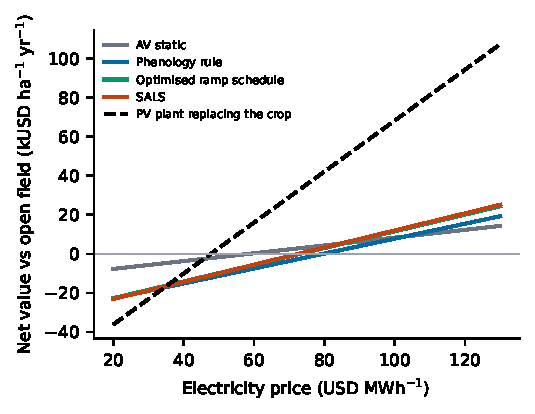
\includegraphics[width=0.48\textwidth]{figures/cost_price.pdf}\hfill
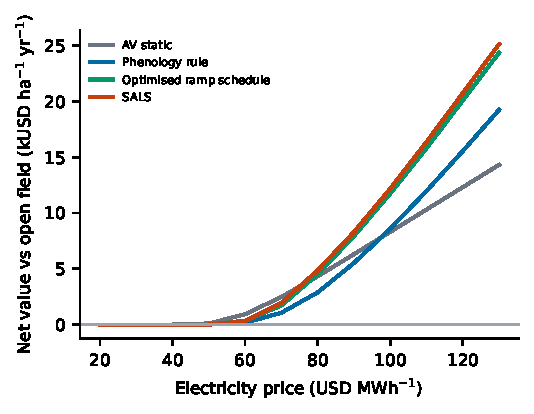
\includegraphics[width=0.48\textwidth]{figures/cost_optimal.pdf}
\caption{Net value per hectare relative to the open field against electricity price. Left: densities designed for the floor, with a conventional plant replacing the crop (dashed). Right: each site chooses the feasible density that maximises its historical net value. Illustrative parameters of Table~\ref{tab:costparams}.}
\label{fig:cost}\label{fig:costopt}
\end{figure}

\textbf{Cost of the safety margin.} At 90\,USD\,MWh$^{-1}$, moving from a density designed under the mean response to a floor of 0.92 under that response costs 1.00 kUSD\,ha$^{-1}$\,yr$^{-1}$ (17\%) under E2 for 18 more points of compliance (70\% to 88\%) and 1.13 kUSD (20\%) under E3 for 14 points (71\% to 85\%), about 56 and 79 USD\,ha$^{-1}$\,yr$^{-1}$ per point. The ensemble rule that requires all other members to meet the floor costs 0.85 and 1.22 kUSD for 19 and 17 points (45 and 74 USD per point), so on this measure it is cheaper than the margin under E2 and similar under E3. At 60\,USD\,MWh$^{-1}$ a margin has a negative cost, because every module beyond break-even loses money; the economics of the design margin therefore depend on the price level, whereas its effect on compliance does not.

\subsection{Agrivoltaics under warming}
Under warming, the open-field production of the held-out sites (Fig.~\ref{fig:warming}) falls at +3\,\textdegree C by 23\% for maize and 18\% for rice, is nearly unchanged for soybean, and rises for wheat (+3\%) and potato (+10\%). Agrivoltaic production with light-sharing control follows the open field at about 90\% of its level, so it inherits the same climate impacts (maize $-31$\%, rice $-27$\% relative to the baseline open field at +3\,\textdegree C). Agrivoltaics does not protect staple production against warming in this model. The LER of light-sharing systems, which is relative to the open field under the same climate, increases slightly with warming (SALS 1.270 to 1.297; phenology rule 1.236 to 1.265), because the floor allows slightly denser arrays in warmer conditions (GCR 0.173 to 0.177 and electricity 510 to 540\,MWh\,ha$^{-1}$\,yr$^{-1}$). The margin of SALS over the rules does not grow with warming (Table~\ref{tab:stats}).

\begin{figure}[t]
\centering
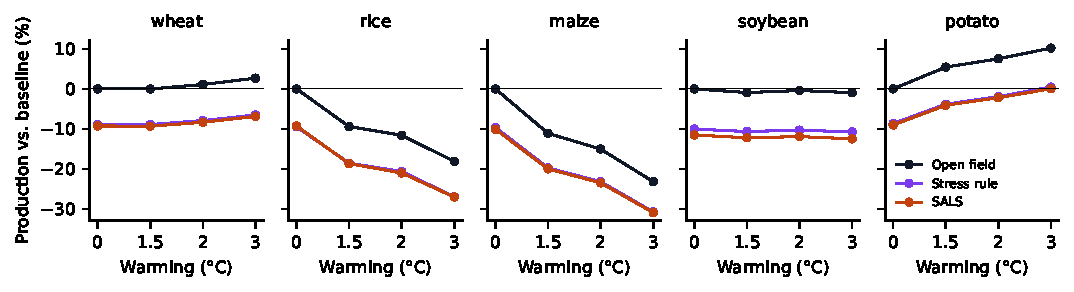
\includegraphics[width=\textwidth]{figures/warming.pdf}
\caption{Production relative to the baseline open field (sum over held-out site-seasons) as a function of warming, for the open field, the stress rule and SALS.}
\label{fig:warming}
\end{figure}

\subsection{Global potential and what it would take}\label{sec:global}
Every site is evaluated when it is held out (222 of the 400 crop--site pairs are held out in at least one split, and three of them have no valid season, leaving 219), and each crop's mean electricity per hectare is scaled to its physical area in SPAM 2010 (581\,Mha for the five crops, which avoids counting multiple-cropped land twice). Equipping 5\% of this area (29.1\,Mha) with SALS arrays at the floor would produce 14.4\,PWh\,yr$^{-1}$ under the baseline climate and 16.0\,PWh\,yr$^{-1}$ at +3\,\textdegree C, with a production-weighted retention of 0.903 and 0.900. The phenology rule would give 13.0 and 14.5\,PWh\,yr$^{-1}$, and static arrays 6.4 and 6.9\,PWh\,yr$^{-1}$. For comparison, world electricity generation was about 30\,PWh in 2023 \citep{ember2024}.

These numbers require large amounts of hardware. SALS at 5\% coverage needs 10.6\,TWp of modules (11.3\,TWp at +3\,\textdegree C), at a capacity factor of 15.5\% (16.2\%). World solar PV capacity at the end of 2024 was about 1.9\,TW \citep{irena2025}, so the requirement is about 5.6 times the installed PV fleet. The electricity is also variable, peaks at midday and would be curtailed or stored. The figures are technical potentials, not projections. Ordering sites by electricity per hectare gives a supply curve (Fig.~\ref{fig:supply}): the best 2\% of the staple cropland would supply about 20\,PWh\,yr$^{-1}$ and the best 4.7\% about 40\,PWh\,yr$^{-1}$ with SALS; this is a ranking of sites by electricity per hectare and not a siting scenario, and it excludes grid, curtailment and land access. The best tenth of the sites are mostly rainfed maize and soybean sites in the Americas and in southern and eastern Africa (7\% mean irrigated fraction against 29\% overall), which are also among the regions where the floor is hardest to meet (Section~\ref{sec:crops}). Siting by electricity alone would therefore concentrate agrivoltaics where food-security risk is highest.

Maize and soybean, for which the simulated shade response is milder than the meta-analysis (Section~\ref{sec:mlresults}), account for 53\% of the electricity of the upscaling (a scaling convention of 5\% of the cropland, reported without an interval) (maize 30\%, soybean 23\%, wheat 29\%, rice 15\%, potato 3\%). Counting only wheat, rice and potato would give about 7\,PWh\,yr$^{-1}$ at the same coverage, so the global figure should be read as an upper estimate for about half of its content. By crop, the LER of SALS under the baseline climate is 1.20 for wheat and rice, 1.31 for potato, 1.30 for maize and 1.41 for soybean.

\begin{figure}[t]
\centering
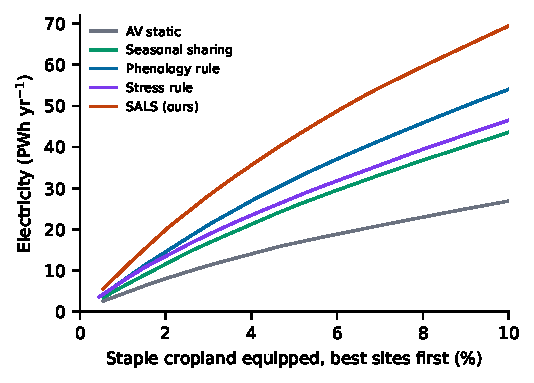
\includegraphics[width=0.6\textwidth]{figures/supply.pdf}
\caption{Supply curve under the baseline climate: cumulative electricity when sites are equipped in order of decreasing electricity per hectare, against the share of staple cropland (physical area) equipped. Each controller is evaluated at the density that keeps its mean retention at 0.9.}
\label{fig:supply}
\end{figure}

\begin{figure}[t]
\centering
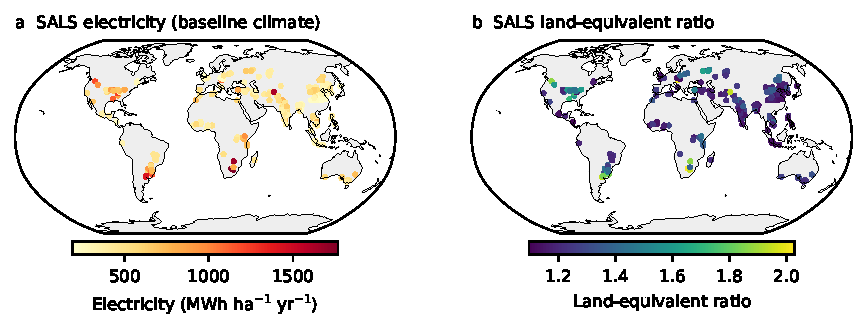
\includegraphics[width=\textwidth]{figures/map.pdf}
\caption{SALS electricity (a) and land-equivalent ratio (b) at the pooled held-out sites (baseline climate, mean of seasons 2015--2019).}
\label{fig:global}
\end{figure}

\subsection{Floor conditioning, chance-constrained training and forecast errors}\label{sec:extra}
\textbf{One network for all floors.} Regulations and farmers set different floors. The network of the main experiments was trained at $\rho=0.9$ only. We evaluated it at floors of 0.80, 0.85, 0.90 and 0.95, re-running the historical design step for each floor (Table~\ref{tab:rho}). Its LER exceeds that of the phenology rule by 0.037, 0.036, 0.034 and 0.033 under the baseline climate (0.040, 0.037, 0.032 and 0.033 at +3\,\textdegree C), so the benefit carries over to other floors without retraining. A network that received the floor as an additional input and was trained over all four floors did not improve on it (differences in LER $\le0.001$). Because the design step already adapts the density to the floor, conditioning the controller on the floor is not needed.

\begin{table}[t]
\centering
\caption{LER of the controllers at different yield-retention floors $\rho$ (main split; the historical design step is repeated for each floor).}
\label{tab:rho}
\small
\setlength{\tabcolsep}{4pt}
\begin{tabular}{lcccccccc}
\toprule
 & \multicolumn{4}{c}{Baseline climate} & \multicolumn{4}{c}{+3\,\textdegree C}\\
\cmidrule(lr){2-5}\cmidrule(lr){6-9}
Method & 0.80 & 0.85 & 0.90 & 0.95 & 0.80 & 0.85 & 0.90 & 0.95\\
\midrule
AV static & 1.159 & 1.115 & 1.072 & 1.011 & 1.174 & 1.128 & 1.083 & 1.013\\
Stress rule & 1.380 & 1.282 & 1.182 & 1.077 & 1.364 & 1.269 & 1.172 & 1.071\\
Phenology rule & 1.467 & 1.356 & 1.236 & 1.108 & 1.513 & 1.395 & 1.265 & 1.122\\
SALS (trained at $\rho=0.9$) & 1.505 & 1.392 & 1.270 & 1.141 & 1.553 & 1.432 & 1.297 & 1.154\\
SALS conditioned on $\rho$ & 1.504 & 1.391 & 1.269 & 1.141 & 1.553 & 1.431 & 1.296 & 1.154\\
\bottomrule
\end{tabular}
\end{table}

\textbf{Layout, rotation limit and harvest-index assumptions.} We checked three assumptions that could drive the ranking (Table~\ref{tab:physsens}; 21 pairs of the main split, one training seed). The rotation limit of the trackers sets how much light sharing can deliver: with a limit of 45$^\circ$ the LER of the phenology rule is 1.138, with 60$^\circ$ 1.170 and with 80$^\circ$ 1.206, whereas static trackers stay at 1.05--1.06, so the benefit of light sharing grows with the limit and the ranking is unchanged. Fixed non-tracking arrays held flat or rotated by 30$^\circ$ about the north--south axis (facing east, not the equator; equator-facing tilts are not modelled) do no better than static trackers (LER 1.048 and 1.043 against 1.053; differences of 0.005 are within the noise of 21 pairs and one training seed), so static trackers are no worse than the fixed arrays we tested; vertical bifacial layouts are not modelled. The ranking of the rules also does not depend on the assumed harvest-index penalty. The window test is weakly informative about the timing of the phenology rule, which shares light through almost the whole growing period, so a shifted window cannot move it much; the informative case is the removal of the penalty. Moving the critical window to 0.30--0.50 or 0.60--0.80 of the thermal-time requirement changes the LER of the phenology rule by at most 0.001, and removing the penalty altogether raises all light-sharing LERs (phenology rule 1.328, SALS 1.353) without changing the order: the phenology rule exceeds seasonal sharing by 0.03 to 0.05 in every case (0.035 with the early window, 0.034 with the late window, 0.053 without penalty), because it produces electricity before canopy development and after maturity, when the crop does not use the light, and not because of the assumed window. The margin of SALS over the written rule changes with these assumptions (0.005 to 0.025 LER), and its margin over the tuned rule is 0.000 to 0.009 (at a rotation limit of 45$^\circ$ SALS equals the tuned rule).

\begin{table}[t]
\centering\small
\caption{Sensitivity of the controller comparison to the rotation limit of the trackers and to the harvest-index penalty (LER; main split, every sixth held-out pair, 21 pairs, main shade response, history-based design on a GCR grid with step 0.05). SALS was trained for the main setting. Fixed arrays (no tracking; flat and tilted by 30$^\circ$ from the horizontal about the north--south axis) reach LER 1.048 and 1.043 in the same sample, against 1.053 for static trackers.}\label{tab:physsens}
\resizebox{\ifdim\width>\linewidth\linewidth\else\width\fi}{!}{\begin{tabular}{lcccc}
\toprule
Setting & Static tracker & Phenology rule & Grid-tuned window & SALS\\
\midrule
Main (limit 60$^\circ$, window 0.45--0.65) & 1.053 & 1.170 & 1.180 & 1.189\\
Rotation limit 45$^\circ$ & 1.057 & 1.138 & 1.144 & 1.144\\
Rotation limit 80$^\circ$ & 1.053 & 1.206 & 1.219 & 1.224\\
Window 0.30--0.50 & 1.053 & 1.169 & 1.176 & 1.185\\
Window 0.60--0.80 & 1.053 & 1.171 & 1.181 & 1.182\\
No harvest-index penalty & 1.109 & 1.328 & 1.347 & 1.353\\
\bottomrule
\end{tabular}}
\end{table}


\textbf{A floor of 66\%.} The German pre-standard DIN SPEC 91434 requires 66\% of the reference yield \citep{din2021}. Repeating the design step with $\rho=0.66$ (baseline climate, main split, same network trained at 0.9) the ground coverage cap of 0.5 binds for the sharing methods (mean GCR 0.48 for the phenology rule and 0.48 for SALS, 0.44 for the stress rule), static arrays reach a coverage of 0.24 and LER 1.28, the phenology rule 1.66 and SALS 1.71. At this floor the density is limited by the cap and by the mean retention of 0.73 reached at the cap, not by the floor, so the comparison of controllers says little about control; we do not interpret it further.

\textbf{Chance-constrained training.} We also trained a network whose objective penalises a batch share of seasons below the floor that exceeds 20\%. It did not improve the tail. With the mean-based design step its LER was 1.263 (baseline) and 1.290 (+3\,\textdegree C) against 1.270 and 1.297, and with chance-constrained design it reached season-level compliance of 92.6\% against 92.0\% and an LER of 1.198 against 1.205. The season-level guarantee is obtained by the design step (Section~\ref{sec:main}), not by the training objective.

\textbf{Forecast errors.} We raised the forecast errors seen by the controllers to 0, 1, 2 and 3 times the errors used in training. The LER of SALS and of the phenology rule was identical at all four error levels to three decimals (densities 0.2 and 0.3: SALS 1.307 and 1.457, phenology rule 1.278 and 1.416). Neither controller uses the weather forecast: both rely on the crop's thermal time, which is observable from on-farm temperature records. The stress rule, which depends on the forecast of maximum temperature, degrades with forecast error: at density 0.3 its retention falls from 0.778 to 0.751 and its LER from 1.432 to 1.418 as the errors triple.

\renewcommand{\appendix}{}
\appendix
\section{Statistical comparison}\label{app:stats}
\begin{table}[h]
\centering
\caption{Paired comparison of SALS with each baseline on the 92 held-out sites of the main split (unit of analysis: site mean over test seasons). $\Delta$LER: mean difference (SALS minus baseline) with cluster-bootstrap 95\% CI; $p$: two-sided Wilcoxon signed-rank test; \% better: share of sites where SALS has the higher LER; $\Delta r$: difference in mean yield retention with its Wilcoxon $p$-value.}
\label{tab:stats}
\scriptsize
\setlength{\tabcolsep}{3pt}
\begin{tabular}{llccccccc}
\toprule
Climate & Baseline & $\Delta$LER [95\% CI] & $p$ & \% better & $\Delta r$ & $p$ & Sites\\
\midrule
Baseline & AV static & +0.205 [+0.176, +0.236] & $<10^{-4}$ & 100 & -0.011 & $<10^{-4}$ & 92\\
Baseline & Seasonal sharing & +0.088 [+0.068, +0.109] & $<10^{-4}$ & 97 & +0.001 & 0.922 & 92\\
Baseline & Phenology rule & +0.038 [+0.025, +0.053] & $<10^{-4}$ & 84 & +0.001 & 0.723 & 92\\
Baseline & Stress rule & +0.096 [+0.071, +0.124] & $<10^{-4}$ & 93 & -0.002 & 0.055 & 92\\
+1.5\,\textdegree C & AV static & +0.208 [+0.180, +0.237] & $<10^{-4}$ & 100 & -0.010 & $<10^{-4}$ & 92\\
+1.5\,\textdegree C & Seasonal sharing & +0.095 [+0.077, +0.114] & $<10^{-4}$ & 98 & +0.001 & 0.812 & 92\\
+1.5\,\textdegree C & Phenology rule & +0.033 [+0.022, +0.045] & $<10^{-4}$ & 86 & +0.002 & 0.855 & 92\\
+1.5\,\textdegree C & Stress rule & +0.108 [+0.083, +0.134] & $<10^{-4}$ & 98 & -0.001 & 0.041 & 92\\
+2\,\textdegree C & AV static & +0.209 [+0.181, +0.238] & $<10^{-4}$ & 100 & -0.010 & $<10^{-4}$ & 92\\
+2\,\textdegree C & Seasonal sharing & +0.097 [+0.079, +0.115] & $<10^{-4}$ & 97 & +0.001 & 0.876 & 92\\
+2\,\textdegree C & Phenology rule & +0.032 [+0.022, +0.044] & $<10^{-4}$ & 85 & +0.002 & 0.496 & 92\\
+2\,\textdegree C & Stress rule & +0.115 [+0.089, +0.142] & $<10^{-4}$ & 98 & -0.003 & 0.016 & 92\\
+3\,\textdegree C & AV static & +0.219 [+0.190, +0.250] & $<10^{-4}$ & 100 & -0.009 & $<10^{-4}$ & 92\\
+3\,\textdegree C & Seasonal sharing & +0.108 [+0.089, +0.129] & $<10^{-4}$ & 96 & +0.001 & 0.935 & 92\\
+3\,\textdegree C & Phenology rule & +0.034 [+0.022, +0.046] & $<10^{-4}$ & 86 & +0.002 & 0.330 & 92\\
+3\,\textdegree C & Stress rule & +0.131 [+0.102, +0.162] & $<10^{-4}$ & 98 & -0.002 & 0.142 & 92\\
\bottomrule
\end{tabular}
\end{table}


\section{Design under shade-response uncertainty: conformal and learned margins}\label{sec:supp-design}
\emph{Conformal risk control.} For each pair, the loss of a margin $d$ is the share of the held-out members under which the pair's mean test retention is below 0.9 (members 0, 3, 5, 8 and 10 of ensemble E2; the design belief is the mean of the other four). A margin is calibrated on the pairs of the two splits that are not the test split, excluding any pair that is also held out in the test split (a pair can be held out in several splits), by the smallest $d$ on a grid from 0.90 to 0.975 (step 0.005) with $n/(n+1)\,\hat R(d)+1/(n+1)\le\alpha$, $n$ the number of calibration pairs; the guarantee concerns the expected loss for a new pair, that is the average over members, and assumes exchangeable pairs, which spatial blocks and shared years only approximate. Table~\ref{tab:supconformal} gives the margins and the results by split. \emph{Learned design.} The network of Table~\ref{tab:suplearned} chooses among the ten densities of the grid (0.05 to 0.50) or no array; its inputs are, at each density, the mean, minimum and maximum over the other four members of the historical (2001--2014) mean retention, together with a crop indicator and the absolute latitude, and its loss is the expected value over the softmax of $-\mathrm{LER}+\lambda\,\mathbf{1}[r<0.9]$ under the held-out member; the decision is the argmax. Because the network sees the spread between members and the margins see only their mean, the comparison is not between identical information; the margins have one parameter that is read off the test results and the network is fitted on training pairs, and the comparison favours the margins in that respect. The oracle (design under the true response) reaches 86.6\% of pairs at the floor and an LER of 1.486 inside the ensemble and 87.8\% and 1.283 outside it. The numbers of this section come from the re-run of the pipeline described in the main text.
\begin{table}[t]
\centering\small
\caption{Conformal margins by test split (ensemble E2): target compliance, test split, number of calibration pairs (pairs of the other two splits that are not in the test split), calibrated margin $d$, number of test pairs, compliance and LER of the test pairs inside the ensemble, and compliance outside the ensemble.}\label{tab:supconformal}
\begin{tabular}{lccccccc}
\toprule
Target & Split & Cal. pairs & $d$ & Test pairs & Inside (\%) & LER & Outside (\%)\\
\midrule
90\% & 0 & 44 & 0.925 & 32 & 89.4 & 1.399 & 34.4\\
90\% & 1 & 50 & 0.930 & 26 & 94.6 & 1.465 & 37.5\\
90\% & 2 & 41 & 0.930 & 35 & 97.1 & 1.358 & 37.9\\
85\% & 0 & 44 & 0.915 & 32 & 82.5 & 1.432 & 29.7\\
85\% & 1 & 50 & 0.920 & 26 & 90.8 & 1.497 & 35.6\\
85\% & 2 & 41 & 0.925 & 35 & 93.7 & 1.378 & 37.1\\
80\% & 0 & 44 & 0.915 & 32 & 82.5 & 1.432 & 29.7\\
80\% & 1 & 50 & 0.915 & 26 & 87.7 & 1.514 & 30.8\\
80\% & 2 & 41 & 0.915 & 35 & 87.4 & 1.406 & 35.7\\
\bottomrule
\end{tabular}
\end{table}

\begin{table}[t]
\centering\small
\caption{Learned design network (one hidden layer of 32 units, 400 full-batch Adam steps at a learning rate of 0.01 with weight decay $10^{-3}$, inputs standardised on the training pairs, three seeds): compliance and LER of the pairs (mean over seeds, splits and held-out members or responses), and LER minus that of the fixed-margin frontier at the same compliance with a 95\% cluster-bootstrap interval over pairs (500 resamples). Negative values mean that the network is worse than a margin. The network has the inputs described in the main text and is trained on the pairs of two splits that are not in the test split.}\label{tab:suplearned}
\begin{tabular}{lcccc}
\toprule
Truth & $\lambda$ & Pairs at floor (\%) & LER & LER minus margin frontier\\
\midrule
inside & 0.5 & 44.4 & 1.645 & --\\
inside & 0.6 & 75.1 & 1.456 & -0.020 (-0.037, -0.003)\\
inside & 0.7 & 81.8 & 1.414 & -0.038 (-0.056, -0.023)\\
inside & 0.8 & 84.2 & 1.401 & -0.044 (-0.061, -0.024)\\
inside & 0.9 & 84.9 & 1.385 & -0.058 (-0.077, -0.036)\\
inside & 1 & 86.7 & 1.378 & -0.057 (-0.076, -0.032)\\
inside & 1.25 & 91.2 & 1.355 & -0.055 (-0.079, -0.032)\\
inside & 1.5 & 94.2 & 1.342 & -0.054 (-0.076, +0.015)\\
inside & 2 & 96.7 & 1.330 & -0.009 (-0.071, +0.070)\\
inside & 3 & 97.6 & 1.320 & +0.009 (-0.070, +0.077)\\
outside & 0.5 & 19.8 & 1.568 & --\\
outside & 0.6 & 30.8 & 1.395 & -0.001 (-0.027, +0.021)\\
outside & 0.7 & 34.8 & 1.359 & -0.009 (-0.028, +0.014)\\
outside & 0.8 & 35.1 & 1.345 & -0.020 (-0.038, -0.001)\\
outside & 0.9 & 36.3 & 1.330 & -0.028 (-0.049, -0.007)\\
outside & 1 & 36.2 & 1.328 & -0.031 (-0.050, -0.010)\\
outside & 1.25 & 39.3 & 1.307 & -0.037 (-0.055, -0.019)\\
outside & 1.5 & 41.2 & 1.295 & -0.044 (-0.061, -0.027)\\
outside & 2 & 42.5 & 1.285 & -0.051 (-0.067, -0.033)\\
outside & 3 & 44.7 & 1.275 & -0.057 (-0.071, -0.039)\\
\bottomrule
\end{tabular}
\end{table}


\section{Shade-response model, ensembles and economics: further tables}\label{sup:model}
\begin{table}[t]
\centering\small
\caption{Predicting relative yield under shade from 428 observations of 58 studies \citep{laub2022}: leave-one-study-out cross-validation (every study held out once; observations with $s>0$). Covariates: irradiation, climate zone, shade type, intercropping.}\label{tab:mlcv}
\resizebox{\ifdim\width>\linewidth\linewidth\else\width\fi}{!}{\begin{tabular}{lcccc}
\toprule
Model & RMSE & MAE & Median AE & Mean MAE per study\\
\midrule
Proportional loss, $y=1-s$ & 0.430 & 0.305 & 0.210 & 0.224\\
One curve for all crops & 0.372 & 0.265 & 0.193 & 0.208\\
Curve per crop type, no pooling & 0.313 & 0.208 & 0.141 & 0.165\\
Curve per crop type, partial pooling & 0.312 & 0.210 & 0.150 & 0.162\\
Partial pooling + covariates & 0.311 & 0.206 & 0.148 & 0.161\\
Gradient-boosted trees & 0.321 & 0.219 & 0.162 & 0.184\\
\bottomrule
\end{tabular}}
\end{table}

\begin{table}[t]
\centering\small
\caption{Leave-one-study-out prediction error (RMSE of relative yield, observations with $s>0$) by crop type: proportional loss, hierarchical curve with partial pooling, and gradient-boosted trees. The last columns give the difference hierarchical minus proportional with a 95\% cluster-bootstrap interval over studies (negative: hierarchical better).}\label{tab:mlcvtype}
\resizebox{\ifdim\width>\linewidth\linewidth\else\width\fi}{!}{\begin{tabular}{lcccccc}
\toprule
Group & Obs./studies & Proportional & Hierarchical & Boosted trees & Difference & 95\% interval\\
\midrule
C3 cereals & 30/10 & 0.214 & 0.187 & 0.205 & -0.027 & [-0.053, +0.019]\\
Maize & 40/10 & 0.225 & 0.235 & 0.248 & +0.010 & [-0.026, +0.068]\\
Grain legumes & 58/14 & 0.215 & 0.225 & 0.234 & +0.010 & [-0.035, +0.058]\\
Tubers/root crops & 10/2 & 0.250 & 0.254 & 0.257 & +0.004 & [-0.008, +0.053]\\
Four crop types used by the simulator & 138/30 & 0.220 & 0.222 & 0.234 & +0.002 & [-0.023, +0.030]\\
Other types (berries, forages, fruits, vegetables) & 201/29 & 0.528 & 0.361 & 0.369 & -0.167 & [-0.210, -0.115]\\
All types & 339/58 & 0.430 & 0.312 & 0.321 & -0.118 & [-0.158, -0.071]\\
\bottomrule
\end{tabular}}
\end{table}

\begin{table}[t]
\centering\small
\caption{Sensitivity of the deployable light-sharing results to the crop shade response (rule controllers, baseline climate, floor $\rho=0.9$, split~0, every fourth held-out site, 22 sites). Conservative: proportional response (main analysis); calibrated: radiation-use compensation fitted to \citet{laub2022}; field-fitted: fitted to the field trials, maize harvest index unaffected.}\label{tab:variants}
\resizebox{\ifdim\width>\linewidth\linewidth\else\width\fi}{!}{\begin{tabular}{llcccc}
\toprule
Shade response & Method & GCR & $E/E_\mathrm{PV}$ & Retention & LER\\
\midrule
conservative & AV static & 0.06 & 0.15 & 0.92 & 1.07\\
 & Phenology rule & 0.17 & 0.33 & 0.90 & 1.23\\
 & Seasonal sharing & 0.16 & 0.28 & 0.90 & 1.18\\
 & Stress rule & 0.11 & 0.24 & 0.91 & 1.15\\
\midrule
calibrated & AV static & 0.07 & 0.18 & 0.91 & 1.09\\
 & Phenology rule & 0.19 & 0.37 & 0.90 & 1.28\\
 & Seasonal sharing & 0.19 & 0.32 & 0.90 & 1.22\\
 & Stress rule & 0.13 & 0.29 & 0.91 & 1.20\\
\midrule
field-fitted & AV static & 0.16 & 0.41 & 0.91 & 1.32\\
 & Phenology rule & 0.37 & 0.70 & 0.92 & 1.62\\
 & Seasonal sharing & 0.37 & 0.61 & 0.92 & 1.53\\
 & Stress rule & 0.29 & 0.63 & 0.90 & 1.53\\
\bottomrule
\end{tabular}}
\end{table}

\begin{table}[t]
\centering\small
\caption{Shade-response parameters of ensemble E2, calibrated by gradient descent through the simulator to the data-driven curves and the field trials (12 randomised fits; mean $\pm$ s.d.): radiation-use compensation $c$ and multiplier $h$ on the flowering-window harvest-index penalty (1 = assumed value).}\label{tab:posterior}
\resizebox{\ifdim\width>\linewidth\linewidth\else\width\fi}{!}{\begin{tabular}{lcc}
\toprule
Crop & $c$ & $h$ multiplier\\
\midrule
Wheat & 0.91 $\pm$ 0.31 & 0.74 $\pm$ 0.53\\
Rice & 0.61 $\pm$ 0.25 & 0.83 $\pm$ 0.33\\
Maize & 0.14 $\pm$ 0.11 & 0.16 $\pm$ 0.13\\
Soybean & 0.05 $\pm$ 0.09 & 1.66 $\pm$ 0.38\\
Potato & 0.62 $\pm$ 0.20 & 0.90 $\pm$ 0.50\\
\bottomrule
\end{tabular}}
\end{table}

\begin{table}[t]
\centering\small
\caption{One-at-a-time sensitivity of the net value (kUSD\,ha$^{-1}$\,yr$^{-1}$, relative to the open field) at 90\,USD\,MWh$^{-1}$, densities designed for the floor as in the main analysis. In the capex rows the capex of the conventional plant is set to 0.75 times that of the agrivoltaic plant.}\label{tab:costsens}
\begin{tabular}{llcccc}
\toprule
Parameter & Value & Static arrays & Optimised window & SALS & Conventional plant\\
\midrule
Base &  & 6.3 & 7.3 & 7.6 & 55.2\\
AV capex (USD/Wp) & 0.7 & 9.7 & 16.6 & 17.1 & 72.8\\
AV capex (USD/Wp) & 1.5 & 0.6 & -8.2 & -8.2 & 25.8\\
Discount rate & 4\% & 8.0 & 12.0 & 12.4 & 64.1\\
Discount rate & 8\% & 4.4 & 2.1 & 2.4 & 45.4\\
Crop prices & 0.5$\times$ & 6.4 & 7.4 & 7.7 & 57.0\\
Crop prices & 2.0$\times$ & 6.0 & 7.0 & 7.3 & 51.6\\
Electricity price & 60 & 0.3 & -5.6 & -5.6 & 16.0\\
Electricity price & 120 & 12.3 & 20.1 & 20.7 & 94.4\\
\bottomrule
\end{tabular}
\end{table}

\begin{table}[t]
\centering\small
\caption{Design rules outside the ensemble E2 by crop: share of crop--site pairs (\%) with mean retention $\ge0.9$ under the proportional (P), calibrated (C), field-fitted (F) and harsh (H) responses (phenology rule, three splits pooled). The number of pairs is given in parentheses; with 10 to 20 pairs per crop a difference of one pair is 5 to 10 points. Pooled values are in Table~\ref{tab:ooe}.}\label{tab:ooecrop}
\resizebox{\ifdim\width>\linewidth\linewidth\else\width\fi}{!}{\begin{tabular}{llcccc}
\toprule
Crop (pairs) & Design & P & C & F & H\\
\midrule
Wheat (17) & oracle & 100 & 94 & 100 & 94\\
 & mean response & 0 & 0 & 100 & 0\\
 & 75\% of members & 0 & 0 & 100 & 0\\
 & floor 0.92 & 0 & 0 & 100 & 0\\
 & floor 0.96 & 12 & 76 & 100 & 0\\
\addlinespace
Rice (20) & oracle & 90 & 90 & 80 & 85\\
 & mean response & 0 & 0 & 10 & 0\\
 & 75\% of members & 0 & 0 & 40 & 0\\
 & floor 0.92 & 0 & 10 & 60 & 0\\
 & floor 0.96 & 95 & 95 & 100 & 85\\
\addlinespace
Maize (17) & oracle & 76 & 76 & 71 & 65\\
 & mean response & 6 & 6 & 71 & 0\\
 & 75\% of members & 12 & 12 & 82 & 0\\
 & floor 0.92 & 18 & 18 & 82 & 0\\
 & floor 0.96 & 71 & 71 & 94 & 53\\
\addlinespace
Soybean (10) & oracle & 90 & 90 & 90 & 90\\
 & mean response & 90 & 90 & 90 & 90\\
 & 75\% of members & 100 & 100 & 100 & 90\\
 & floor 0.92 & 100 & 100 & 100 & 90\\
 & floor 0.96 & 100 & 100 & 100 & 100\\
\addlinespace
Potato (12) & oracle & 100 & 100 & 100 & 92\\
 & mean response & 0 & 0 & 100 & 0\\
 & 75\% of members & 0 & 0 & 100 & 0\\
 & floor 0.92 & 0 & 0 & 100 & 0\\
 & floor 0.96 & 42 & 42 & 100 & 42\\
\bottomrule
\end{tabular}}
\end{table}


\bibliographystyle{elsarticle-harv}
\bibliography{references}
\end{document}
